\declarecommand\bpnote[1]{\textcolor{blue}{{\textbf{Brandon Says: #1}}}}
\declarecommand\jwnote[1]{\textcolor{purple}{{\textbf{Jingbo Says: #1}}}}
\declarecommand\cwnote[1]{\textcolor{red}{{\textbf{Chao Says: #1}}}}

\declarecommand{\Name}{\textsc{LinSyn}}
\declarecommand{\ReluDiff}{\textsc{ReluDiff}}
\declarecommand{\ReluVal}{\textsc{ReluVal}}
\declarecommand{\DeepPoly}{\textsc{DeepPoly}}
\declarecommand{\Reluplex}{\textsc{Reluplex}}
\declarecommand{\Neurify}{\textsc{Neurify}}
\declarecommand{\Crown}{\textsc{Crown}}
\declarecommand{\Popqorn}{\textsc{Popqorn}}
\declarecommand{\RefineZono}{\textsc{RefineZono}}
\declarecommand{\dReal}{\textsc{dReal}}
\declarecommand{\autolipra}{\textsc{AutoLiRPA}}
\declarecommand{\popqorn}{\textsc{POPQORN}}

% NN verification is important due to adversarial behaviors
Neural networks have become a popular model choice in machine learning due to
their performance across a wide variety of tasks ranging from image
classification~\cite{he2016deep}, natural language
processing~\cite{vaswani2017attention}, and
control~\cite{hu2020reach,JulianKO18}. However, they are also
known to misclassify inputs in the presence of both small amounts of input
noise and seemingly insignificant perturbations to the
inputs~\cite{szegedy2013intriguing}. Indeed, many works have shown they are
vulnerable to a variety of seemingly benign input
transformations~\cite{engstrom2019exploring,kanbak2018geometric,alzantot2018generating},
which raises concerns about their deployment in safety-critical systems.
% Linear approximations have a wide range of applications,
% including NN verification
As a result, a large number of works have proposed verification techniques to
prove that a neural network is not vulnerable to these
perturbations~\cite{SinghGPV19,WangPWYJ18,WengZCSHDBD18}, or in
general satisfies some
specification~\cite{KatzBDJK17,KatzHIJLLSTWZDK19,hu2020reach}. Crucial to the
precision and scalability of these verification techniques are \textit{linear
approximations} of the network's activation functions.


% What is actually the problem?

In essence, given some arbitrary activation function $ \sigma(x) $, a linear
approximation is a \textit{coefficient generator function}
$ \mathcal{G}: (l, u) \to \langle a_l, b_l, a_u, b_u \rangle $, where $ l, u
\in \mathbb{R} $ are real values that correspond to the interval $ [l, u] $,
and $ a_l, b_l, a_u, b_u \in \mathbb{R} $ are real-valued coefficients
in the linear lower and upper bounds such that the following condition holds:
\begin{equation}
\begin{gathered}
\forall x \in [l, u]. \;\; a_l \cdot x + b_l \leq \sigma(x) \leq a_u
\cdot x + b_u
\end{gathered}
\end{equation}
Indeed, a key contribution in many seminal works on neural network verification
was a hand-crafted $ \mathcal{G}(l, u)
$~\cite{SinghGPV19,WangPWYJ18,WangPWYJ18nips,balunovic2019certifying,du2021cert,ko2019popqorn,zhang2018efficient,WengZCSHDBD18,wu2021tightening,ryou2021scalable,shi2020robustness}
and follow-up work built off these
hand-crafted
approximations~\cite{KatzHIJLLSTWZDK19,tjeng2019evaluating,SinghGPV19iclr,Singh2019krelu}.
Furthermore, linear approximations have applications beyond neural network
verification, such as rigorous global optimization and
verification~\cite{lebbah2007efficient,trombettoni2011inner}.

However, crafting $ \mathcal{G}(l, u) $ is tedious, error-prone, and requires
an expert. Unfortunately, in the case of neural network activation functions,
experts have only crafted approximations for the most common functions, namely
ReLU, sigmoid, tanh, max-pooling, and those in vanilla LSTMs. As a result,
existing techniques cannot handle new and cutting-edge activation functions,
such as Swish~\cite{ramachandran2017searching},
GELU~\cite{hendrycks2016gaussian}, Mish~\cite{misra2019mish}, and
LiSHT~\cite{roy2019lisht}.

In this work, we consider the problem of automatically synthesizing the coefficient generator function
$\mathcal{G}(l, u) $, which can alternatively be viewed as four individual
functions $\mathcal{G}_{a_l}(l,u)$, $\mathcal{G}_{b_l}(l,u)$,
$\mathcal{G}_{a_u}(l,u)$, and $\mathcal{G}_{b_u}(l,u)$, one
for each
coefficient.
However, synthesizing the generator functions is a challenging task because (1)
the search space for each function is very large (in fact, technically
infinite), (2) the optimal generator functions are highly nonlinear for all
activation functions considered both in our work and prior work, and (3) to
prove soundness of the synthesized generator functions, we must show:
\begin{equation}
\begin{gathered}\label{offlinesyn:eq:intro-sound}
\forall [l, u] \in \mathbb{IR}, x \in [l, u] ~.\\
(\mathcal{G}_{a_l}(l,u) \cdot x + \mathcal{G}_{b_l}(l,u))
\leq \sigma(x) \leq
(\mathcal{G}_{a_u}(l,u) \cdot x + \mathcal{G}_{b_u}(l,u))
\end{gathered}
\end{equation}
where $ \mathbb{IR} = \{[l, u] ~|~ l, u \in \mathbb{R}, l \leq u \} $ is the
set of all real intervals. The above equation has
highly non-linear constraints, which cannot be directly handled by
standard verification tools, such as the Z3~\cite{de2008z3} SMT solver.

%\textcolor{red}{Synthesizing such generator functions is  a challenging task
%for two reasons.
%%
%First, it is difficult to find generator functions that can produce
%tight linear bounds for a wide range of input intervals.
%%
%Second, it is difficult to prove that the generator functions are
%sound.  While the resulting bounds are linear in terms of $x$, the
%generator functions themselves may be highly non-linear in terms of
%$l$ and $u$.  To ensure that the linear bounds are sound for all
%possible ways of instantiating $l$ and $u$, we must prove the
%soundness of the generator functions as follows:
%%
%\begin{equation}
%\begin{gathered}\label{offlinesyn:eq:intro-sound}
%\forall x \in [l, u]  ~.~
%  (\mathcal{G}_{c^l_1}(l,u) \cdot x + \mathcal{G}_{c^l_2}(l,u))
%  \leq \sigma(x) \leq
%  (\mathcal{G}_{c^u_1}(l,u) \cdot x + \mathcal{G}_{c^u_2}(l,u))
%\end{gathered}
%\end{equation}
%%
%However, such non-linear constraints cannot be directly handled by
%standard verification tools, such as the Z3 SMT solver.
%%
%}


To solve the problem, we propose a novel example-guided synthesis and
verification approach, which is applicable to any differentiable,
Lipschitz-continuous activation function $ \sigma(x) $. (We note that
activation functions are typically required to be differentiable and
Lipschitz-continuous in order to be trained by gradient descent, thus our
approach applies to any \textit{practical} activation function).
%
To tackle the potentially infinite search space of $ \mathcal{G}(l, u) $, we
first propose two \textit{templates} for $ \mathcal{G}(l, u) $, which are
inspired by the hand-crafted coefficient functions of prior work.
%
The ``holes'' in each template are filled by a machine learning model, in our
case a small neural network or linear regression model.
%
Then, the first step is to partition the input space of $ \mathcal{G}(l,
u) $, and then assign a single template to each subset in the partition.
%
The second step is to fill in the holes of each template. Our approach
leverages an example-generation procedure to produce a large number of training
examples of the form $((l, u), (a_l, b_l, a_u, b_u)) $, which can then be used
to train the machine learning component in the template.
%
However, a template instantiated with a trained model may still violate
Equation~\ref{offlinesyn:eq:intro-sound}, specifically the lower bound (resp.
upper bound) may be above (resp. below) the activation function over some
interval $ [l, u] $.
%
To ensure soundness, the final step is to bound the
\textit{maximum violation} of a particular template instance using a rigorous
global optimization technique based on interval analysis, which is implemented
by the tool IbexOpt~\cite{chabert2009contractor}.
%
We then use the computed maximum violation to adjust the template to ensure
Equation~\ref{offlinesyn:eq:intro-sound} always holds.

\begin{figure}[t]
\centering
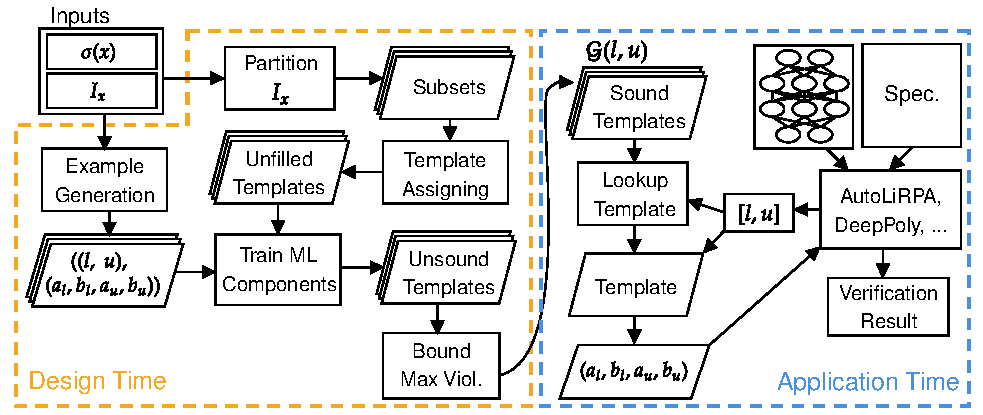
\includegraphics[width=.95\linewidth]{offlinesyn/figs/flow.pdf}
\caption{Overview of our method for synthesizing the \emph{coefficient generator
function}.}
\label{offlinesyn:fig:overview}
\end{figure}

The overall flow of our method is shown in Figure~\ref{offlinesyn:fig:overview}.
%
It takes as input the activation function $ \sigma(x) $, and the set of input
intervals $ I_x \subseteq \mathbb{IR} $ for which $ \mathcal{G}(l, u) $ will be
valid.
%
During \textit{design time}, we follow the previously described approach, which
outputs a set of sound, instantiated templates which make up $ \mathcal{G}(l,
u) $. Then the synthesized $ \mathcal{G}(l, u) $ is integrated into an existing
verification tool such as~\autolipra{}~\cite{autolipra}
or~\DeepPoly{}~\cite{SinghGPV19}.
These tools take as input a neural network and a specification, and output the
verification result (proved, counterexample, or unknown).
%
At \textit{application time} (i.e., when attempting to verify the input
specification), when these tools need a linear approximation for
$ \sigma(x) $ over the interval $ [l, u] $, we lookup the appropriate template
instance, and use it to compute the linear approximation $(a_l, b_l, a_u, b_u)$,
and return it to the tool.

To the best of our knowledge, our method is the first to synthesize a linear
approximation generator function $ \mathcal{G}(l, u) $ for any given activation function $ \sigma(x)
$. Our approach is fundamentally different from the ones used by state-of-the-art neural network verification tools such as~\autolipra{}
and~\DeepPoly{}, which require an expert to hand-craft the approximations. We
note that, while~\autolipra{} can handle activations that it does not
explicitly support by \textit{decomposing} $ \sigma(x) $ into
elementary operations for which it has (hand-crafted) linear approximations,
and then combining them, the resulting bounds are often not tight.
In contrast, our method synthesizes linear approximations for $
\sigma(x) $ as a whole, and we show experimentally that our synthesized
approximations significantly outperform~\autolipra{}.

%We note that our method is fundamentally different from existing approaches
%such as~\DeepPoly{}~\cite{SinghGPV19},~\autolipra{}~\cite{autolipra},
%and~\popqorn{}.
%Our method is fundamentally different from existing approaches adopted
%by tools
%%
%\textcolor{red}{
%%
%such as \DeepPoly{}, \popqorn{} and \autolipra{}.
%%
%Specifically, \DeepPoly{} ...
%%
%\popqorn{}...
%%
%\autolipra{}...
%%
%In contrast, our method synthesizes a \emph{bounds-generating
%function} capable of producing sound and tight linear bounds at run
%time for any concrete interval $[l,u]$.
%%
%}


We have implemented our approach and evaluated it on popular neural
network verification problems (specifically, robustness verification problems in the presence of input perturbations).
Compared against state-of-the-art linear approximation based
verification tools, our synthesized linear approximations can drastically
outperform these existing tools in terms of the number of problems verified on
recently published activation functions such as Swish~\cite{ramachandran2017searching},
GELU~\cite{hendrycks2016gaussian}, Mish~\cite{misra2019mish}, and
LiSHT~\cite{roy2019lisht}.

To summarize, we make the following contributions:
\begin{itemize}
	\item We propose the first method for synthesizing the linear
	approximation generator function $ \mathcal{G}(l, u) $ for any given activation function.
	\item We implement our method, use it to synthesize linear approximations
	for several novel activation functions, and integrate these approximations
	into a state-of-the-art neural network verification tool.
	\item We evaluate our method on a large number of neural network
	verification problems, and
	show that our synthesized approximations significantly outperform
	the state-of-the-art tools.
\end{itemize}



\section{Preliminaries}
\label{offlinesyn:sec:preliminaries}

In this section, we discuss background knowledge necessary to understand our
work. Throughout the paper, we will use the following notations: for variables or scalars we use lower
case letters (e.g., $ x \in \mathbb{R} $), for vectors we use bold lower case
letters (e.g., $ \mathbf{x} \in \mathbb{R}^n $) and for matrices we use bold
upper case letters (e.g., $ \mathbf{W} \in \mathbb{R}^{n \times m} $). In
addition, we use standard interval notation: we let $ [l,u] = \{x \in
\mathbb{R}| l \leq x \leq u \} $ be a real-valued interval, we denote the set
of all real intervals as $
\mathbb{IR} = \{[l,u] | l, u \in \mathbb{R}, l \leq u\} $, and finally we
define the set of $ n $-dimensional intervals as
$ \mathbb{IR}^n = \{
\bigtimes_{i=1}^n [l_i, u_i] \; | \; [l_i, u_i] \in \mathbb{IR} \} $, where $
\bigtimes $ is the Cartesian product.

\subsection{Neural Networks}

We consider a neural network to be a function $ f: \mathbb{X} \subseteq
\mathbb{R}^n \to \mathbb{Y} \subseteq \mathbb{R}^m $, which has $ n $ inputs
and $ m $ outputs.
%
\begin{comment}
$ \mathbb{X} $ may be, for example, the set of all images, and an
input $ \mathbf{x} \in \mathbb{X} $ would be the pixels of an image
flattened into a vector. We focus on neural networks classifiers where
each element in the output vector $ f(\mathbf{x})
\in \mathbb{Y} $ represents a score for one of $ m $ classes, and the highest
score is the predicted class.
\end{comment}
%
For ease of presentation, we focus the discussion
on \textit{feed-forward, fully-connected} neural networks (although
the bounds synthesized by our method apply to all neural
network architectures).
%
For $ \mathbf{x} \in \mathbb{X} $, such networks compute $ f(\mathbf{x}) $ by
performing an alternating
series of matrix multiplications followed by the element-wise
application of an activation function $
\sigma(x) $.


Formally, an $ l $-layer neural network with $ k_i $ neurons in each
layer (and letting $ k_0 = n, k_l = m $) has $ l $ weight matrices
and bias vectors $ \mathbf{W}_i \in \mathbb{R}^{k_{i-1} \times k_i} $
and $ \mathbf{b}_i
\in \mathbb{R}^{k_{i}} $ for $ i \in \{1..l\} $. The input of the network is $
f_0 =
\mathbf{x}^T $, and the output of layer $ i $ is given by the function:
$ f_i = \sigma(f_{i-1} \cdot \mathbf{W}_i + \mathbf{b}_i) $
which can be applied recursively until the output layer of the network is reached.

Initially, common choices for the activation function $ \sigma(x) $ were $ ReLU(x) = max(0, x) $, $
sigmoid(x) = \frac{e^x}{e^x + 1} $, and $ tanh(x) = \frac{e^x - e^{-x}}{e^x +
e^{-x}}  $, however the field has advanced rapidly in recent years and, as a result,
automatically discovering novel activations has become a
research subfield of its own~\cite{ramachandran2017searching}. Many recently proposed activations,
such as Swish and GELU~\cite{ramachandran2017searching,hendrycks2016gaussian},
have been shown to outperform the common choices in important machine learning tasks.


\subsection{Existing Neural Network Verification Techniques and Limitations}

We consider neural network verification problems of the following form: given a neural
network $ f : \mathbb{X} \to \mathbb{Y} $ and an input set $ X \subseteq
\mathbb{X} $, compute an over-approximation $ Y $ such that $ \{f(\mathbf{x}) \mid
\mathbf{x} \in X \} \subseteq Y \subseteq \mathbb{Y} $.
%
The most scalable approaches to neural network verification
(where scale is measured by number of neurons in the network)
 use linear bounding techniques to compute
$ Y $, which require a \textit{linear approximation} of the network's
activation function.
%
This is an extension of \textit{interval
analysis}~\cite{moore2009introduction} (e.g., intervals with linear
lower/upper bounds~\cite{SinghGPV19,autolipra}) to compute $ Y $, and thus
$ X $ and $ Y $ are represented as elements of $
\mathbb{IR}^n $ and $ \mathbb{IR}^m $, respectively.

\begin{comment}
In classification, we are typically interested in showing that for
some set of inputs $ X \subseteq
\mathbb{R} $, $ f $ always produces the same classification. If $ j \in
\{1..m\} $ is the target class, and we
compute $ Y = \bigtimes_{i=1}^m [l_i, u_i] $, then this amounts to checking
that $ l_j > u_i, i \neq j, i \in \{1..m\} $ (i.e., class $ j $'s lower bound is
greater than all other classes upper bound).
\end{comment}

We use Figure~\ref{offlinesyn:fig:motex} to illustrate a typical neural network
verification problem.
The network has input neurons $ x_1, x_2 $,
output neurons $ x_7, x_8 $ and a single hidden layer. We assume the activation
function is $ swish(x) = x \cdot sigmoid(x) $, which is shown by the blue line
in Figure~\ref{offlinesyn:fig:motex-linapprox}. Our input space is $ X = [-1, 1]
\times
[-1, 1] $ (i.e., $ x_1, x_2 \in [-1, 1] $), and we want to prove  $
x_7 > x_8 $, which can be accomplished by first computing the bounds $ x_7 \in [l_7, u_7],
x_8 \in [l_8, u_8] $, and then showing $ l_7 > u_8 $. Following the prior
work~\cite{SinghGPV19} and for simplicity, we split the affine transformation
and application of activation function in the hidden layer into two steps, and we assume the
neurons $ x_i$, where $i \in \{1..8\} $, are ordered such that $ i < j $ implies that $
x_i $ is in either the same layer as $ x_j $, or a layer prior to $ x_j $.

\begin{figure}[t]
\centering
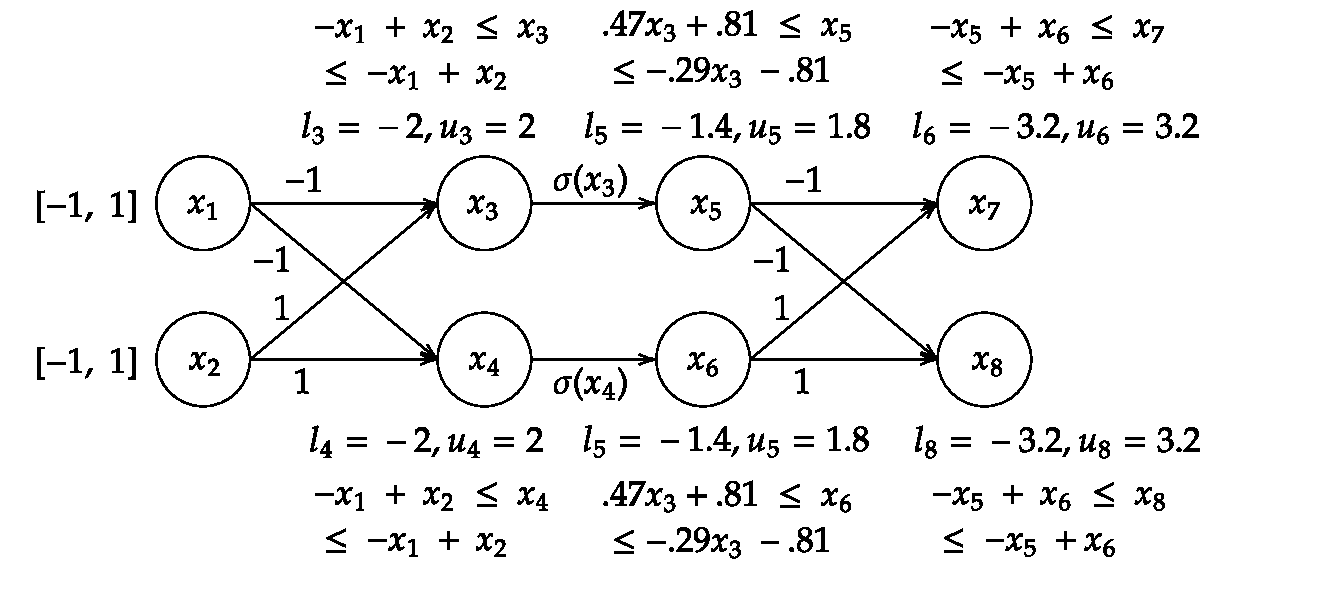
\includegraphics[width=0.9\linewidth]{offlinesyn/figs/motex.pdf}
\caption{An example of linear bounding for neural network verification.
\label{offlinesyn:fig:motex}}
\end{figure}

Linear bounding based neural network verification techniques work as follows.
For each neuron $
x_i $, they compute the concrete lower and upper bounds $ l_i$ and $u_i $,
together with symbolic
lower and upper bounds.  The symbolic lower and upper bounds are linear constraints $
\sum_{j=0}^{i-1} c^l_j \cdot x_j + c^l_i \leq x_i \leq \sum_{j=0}^{i-1} c^u_j
\cdot x_j + c^u_i $, where each of $ c^l_i, c^u_i $ is a constant. Both bounds are
computed in a forward layer-by-layer fashion, using the result of the previous
layers to compute bounds for the current layer.

We illustrate the computation in Figure~\ref{offlinesyn:fig:motex}. In the
beginning, we have $
x_1 \in [-1, 1] $ as the concrete bounds, and $ -1 \leq x_1 \leq 1 $ as the
symbolic  bounds, and similarly for $ x_2 $. To obtain bounds for $ x_3, x_4 $, we
multiply $ x_1, x_2 $ by the edge weights, which for $ x_3 $ gives the linear
bounds $ -x_1 + x_2 \leq x_3 \leq -x_1 + x_2 $ . Then, to compute $ l_3 $ and $
u_3 $, we minimize and maximize the linear lower and upper bounds,
respectively, over $ x_1, x_2 \in [-1, 1] $. Doing so results in $ l_3 = -2,
u_3 = 2 $. We obtain the same result for $ x_4 $.

However, we encounter a key challenge when attempting to bound $ x_5 $, as
we need a linear approximation of $ \sigma(x_3) $ over $ [l_3, u_3] $ when
bounding $ x_5 $, and similarly for $ x_6 $. Here, a linear approximation
for $ x_5 $ can be regarded as a set of coefficients $ a_l, b_l, a_u, b_u $ such that the
following \textit{soundness} condition holds: $ \forall x_3 \in
[l_3, u_3] ~.~ a_l \cdot x_3 + b_l \leq \sigma(x_3) \leq a_u \cdot
x_3 + b_u $.
%
In addition, a sub goal for the bounds is \textit{tightness},
which typically means the volume between the bounds and $ \sigma(x) $ is
minimized.
%
Crafting a function to generate these coefficients has been the
subject of many prior works. Many seminal papers on neural network verification
have focused on solving this problem alone. Broadly speaking, they fall into
the following categories.


\paragraph{Hand-crafted Approximation Techniques} The first category of
techniques use hand-crafted functions for generating $ a_l, b_l, a_u, b_u $.
Hand-crafted functions are generally fast because they are static, and tight
because an expert designed them.
%
Unfortunately, current works in this category are not \textit{general} -- they
only considered the most common activation functions, and thus cannot currently
handle our motivating example or any recent, novel activation functions.
%
For these works to apply to our motivating example, an expert would need to hand-craft an
approximation for the activation function, which is both difficult and error-prone.

\paragraph{Expensive Solver-Aided Techniques}
The second category use expensive solvers and optimization tools to compute
sound and tight bounds in a general way, but at the cost of runtime.
%
Recent works include DiffRNN~\cite{mohammadinejad2020diffrnn} and
POPQORN~\cite{ko2019popqorn}. The former uses (unsound) optimization to
synthesize candidate coefficients and then uses an SMT solver to
verify soundness of the bounds. The latter uses constrained-gradient descent to
compute coefficients. We note that, while these works do not
explicitly target an arbitrary activation function $ \sigma(x) $, their
techniques can be naturally extended.
%
Their high runtime and computational cost are undesirable and, in general, make
them less scalable than the first category.

%\begin{wrapfigure}{R}{0.5\textwidth}
\begin{figure}[t]
	\centering
%	\vspace{-2ex}
	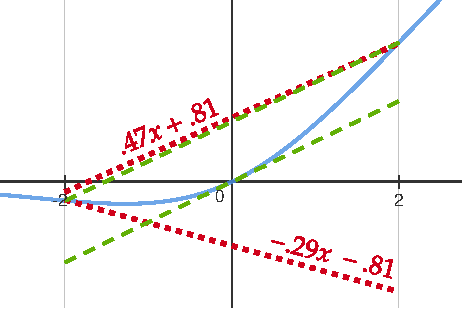
\includegraphics[width=.5\linewidth]{offlinesyn/figs/motex-linapprox.pdf}
	\caption{Approximation of~\autolipra{} (red) and our approach
		(green).\label{offlinesyn:fig:motex-linapprox}}
\end{figure}
%\end{wrapfigure}
\paragraph{Decomposing Based Techniques} The third category combine
hand-crafted approximations with a decomposing based technique to obtain
generality and efficiency, but at the cost of tightness. Interestingly, this is
similar to the approach used by nonlinear SMT solvers and optimizers such as
dReal~\cite{gao2013dreal} and Ibex~\cite{chabert2009contractor}.
%
To the best of our knowledge, only one
work~\autolipra{}~\cite{autolipra} implements this approach for neural network
verification.
%
Illustrating on our example,~\autolipra{} does not have a static linear
approximation for $ \sigma(x_3) = x_3 \cdot sigmoid(x_3) $, but it has
static approximations for $ sigmoid(x_3) $ and $ x_3 \cdot y $.
%
Thus we can
bound $ sigmoid(x_3) $ over $ x_3 \in [-2,2] $, and then, letting $ y =
sigmoid(x_3) $, bound $ x_3 \cdot y $. Doing so results in the approximation
shown as red lines in Figure~\ref{offlinesyn:fig:motex-linapprox}.
%
While useful, they are
suboptimal because they do not minimize the area between the two bounding
lines. This suboptimality occurs due to the decomposing, i.e., the static
approximations used here were not designed for $ swish(x) $ as a whole, but designed
for the individual elementary operations.

\paragraph{Our Work: Synthesizing Static Approximations} Our work overcomes the
limitation of prior work by automatically synthesizing a \textit{static}
function specifically for any given activation function $ \sigma(x) $
\textit{without} decomposing. Since the
synthesis is automatic, and results in a bound generator function, we obtain generality
and efficiency, and since the synthesis targets $ \sigma(x) $ specifically, we
\textit{usually} (demonstrated empirically) obtain tightness.
%
In Figure~\ref{offlinesyn:fig:motex-linapprox}, for example, the bounds computed
by our method are represented by the green lines.
%
The synthesized bound generator function can then be integrated
to state-of-the-art neural network verification tools, including \autolipra{}.

\paragraph{Wrapping Up the Example}
For our running example, using~\autolipra{}'s linear approximation,
we would add the linear bounds for $ x_5 $ shown in
Figure~\ref{offlinesyn:fig:motex}. To
compute $ l_5, u_5 $, we would substitute the linear bounds for $ x_3 $ into $
x_5 $'s linear bounds, resulting in linear bounds with only $ x_1, x_2 $ terms
that can be minimized/maximized for $ l_5, l_6 $ respectively. We do the same
for $ x_6 $, and then we repeat the entire process until the output layer is
reached.

\section{Problem Statement and Challenges}

In this section, we formally define the synthesis problem and then explain the
technical challenges.
%
During the discussion, we focus on synthesizing the generator
functions for the upper bound. We note that we can synthesize lower bound
generator functions analogously.
%

\subsection{The Synthesis Problem}
\label{offlinesyn:sec:synthesis-problem}

Given an activation function $ \sigma(x) $ and an input universe $ x
\in [l_x, u_x] $, we define the set of all intervals over $ x $ in this universe
as $ I_x = \{ \; [l, u] \;|\; [l, u] \in \mathbb{IR}, l, u \in [l_x, u_x] \}$.
(In our experiments, for instance, we use $ l_x = -10$ and $u_x = 10 $).


Our goal is to synthesize a generator function $\mathcal{G}:
(l,u)\to \langle a_u,b_u\rangle$, or equivalently, two generator
functions $\mathcal{G}_{a_u}(l,u)$ and $\mathcal{G}_{b_u}(l,u)$ such that
%
$\forall [l, u] \in I_x, x \in \mathbb{R}$, the condition $
  x \in [l, u] \implies  \sigma(x) \leq \mathcal{G}_{a_u}(l, u) \cdot x
  +\mathcal{G}_{b_u}(l,u)
$ holds.
%
This is the same as requiring that the following condition does
\textbf{not} hold (i.e., the formula is unsatisfiable):
%
\begin{gather*}\label{offlinesyn:eq:sound}
\exists [l, u] \in I_x, x \in \mathbb{R} ~.~ x \in [l, u] \wedge \sigma(x) >
\mathcal{G}_{a_u}(l, u) \cdot x +
\mathcal{G}_{b_u}(l,u)
\end{gather*}
The formula above expresses the search for a counterexample, i.e., an input interval $
[l, u] $ such that $ \mathcal{G}_{a_u}(l, u) \cdot x + \mathcal{G}_{b_u}(l, u)
$ is not a sound upper bound of $\sigma(x) $ over the interval $ [l, u] $.
%
Thus, if the above formula is unsatisfiable, the soundness of the coefficient
functions $ \mathcal{G}_{a_u}, \mathcal{G}_{b_u} $ is proved.
%The first  conjunct ($ l < u $)
%restricts the search space to only valid input intervals. The next two
%conjuncts ($ l \leq x \wedge x \leq u \; $) ensure the validity of the
%counterexample. The last conjunct expresses the unsoundness of the upper bound
%for a given input interval $ [l, u] $ at point $ x $.
%
%Alternatively, we can
%view our goal as finding $ a_u, b_u $ such that the following \textbf{does}
%hold:
%\begin{gather*}
%\forall l \in [l_x, u_x], u \in [l_x, u_x], x \in [l_x, u_x] \\
%l \geq u \vee l > x \vee x > u \; \vee \\
%\sigma(x) \leq a_u(l, u)x + b_u(l, u)
%\end{gather*}

In addition to \textit{soundness}, we want the bound to be \textit{tight},
which in our context has two complementary goals.
%
For a given $ [l, u] \in I_x $ we should have (1) $
\sigma(z) = \mathcal{G}_{a_u}(l, u) \cdot z + \mathcal{G}_{b_u}(l, u) $ for at
least one $ z \in [l, u] $ (i.e., the bound touches $ \sigma(x) $ at
some point $ z $),
%
and (2) the volume below $ \mathcal{G}_{a_u}(l, u) \cdot x +
\mathcal{G}_{b_u}(l, u) $ should be minimized (which we note is equivalent to
minimizing the volume between the upper bound and $\sigma(x)$ since $\sigma(x)$ is fixed).
%
We will illustrate the volume by the shaded green region below the dashed
bounding line in Figure~\ref{offlinesyn:fig:samplelp}.


The first goal is intuitive: if the bound does not touch $
\sigma(x) $, then it can be shifted downward by some constant. The second goal
is a heuristic taken from prior work that has been shown to yield a precise
approximation of the neural network's output set.
%TODO: introduce tightness (in preliminaries?)


\subsection{Challenges and Our Solution}

We face three challenges in searching for the generator functions $
\mathcal{G}_{a_u}$ and $ \mathcal{G}_{b_u} $. First, we must restrict
the search space so that a candidate can be found in a reasonable amount of
time (i.e., the search is tractable). The second challenge, which is at odds
with the first, is that we must have a large enough search space such that it
permits candidates that represent tight bounds.
%If our search space is
%overly-restricted the synthesized $ \mathcal{G}_{a_u}, \mathcal{G}_{b_u} $ may
%be useless.
Finally, the
third challenge, which is at odds with the second, is that we must be able to
formally verify $ \mathcal{G}_{a_u}, \mathcal{G}_{b_u} $ to be sound. While
more complex geneator functions ($ \mathcal{G}_{a_u}, \mathcal{G}_{b_u} $) will
likely
produce tighter bounds, they will be more difficult (if not
impractical) to verify.

%\begin{wrapfigure}{R}{0.5\textwidth}
\begin{figure}[t]
	\centering
%	\vspace{-2ex}
	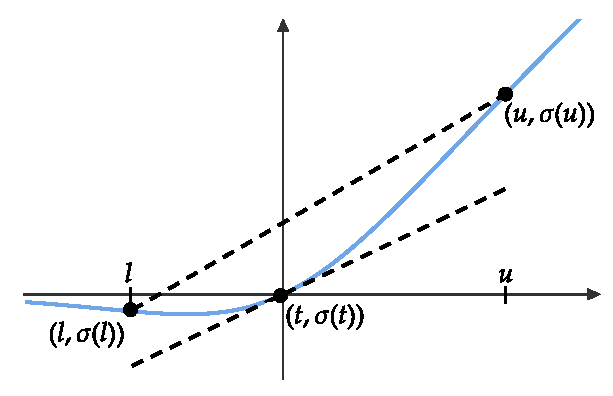
\includegraphics[width=0.5\linewidth]{offlinesyn/figs/twopt_tanpt.pdf}
	\caption{Illustration of the two-point form bound (upper dashed line) and
	tangent-line form bound (lower dashed line).\label{offlinesyn:fig:twopttanpt}}
%	\vspace{-2ex}
\end{figure}
%\end{wrapfigure}
We tackle these challenges by proposing two templates for $ \mathcal{G}_{a_u},
\mathcal{G}_{b_u} $ and then
developing an approach for selecting the appropriate template.
%
We observe that prior work has always expressed the linear bound for $
\sigma(x) $ over an interval $ x \in [l, u] $
%We observe that
%linear bounds of a 1-D activation function $ \sigma(x) $ over a region $ x \in
%[l, u] $ can usually be expressed
as either the line connecting the points $ (l, \sigma(l)), (u, \sigma(u)) $,
referred to as the \textit{two-point form}, or as the line tangent to $
\sigma(x) $ at a point $ t $, referred to as \textit{tangent-line form}.
%
We illustrate both forms in
Figure~\ref{offlinesyn:fig:twopttanpt}.
Assuming that $ \sigma'(x) $ is the derivative of $ \sigma(x) $,
the two templates for $ \mathcal{G}_{a_u}$ and $\mathcal{G}_{b_u} $ as follows:
\begin{align}
\begin{aligned}
&\mathcal{G}_{a_u}(l, u) = \frac{\sigma(u) - \sigma(l)}{u - l} \\
&\mathcal{G}_{b_u}(l, u) = - \mathcal{G}_{a_u}(l, u) \cdot l + \sigma(l) +
\epsilon
\end{aligned} &\hspace{36pt}
\begin{aligned}
\text{two-point}\\
\text{form template}
\end{aligned}
\label{offlinesyn:eq:template-2pt}\\[2ex]
\begin{aligned}
&\mathcal{G}_{a_u}(l, u) = \sigma'(g(l, u)) \\
&\mathcal{G}_{b_u}(l, u) = -\mathcal{G}_{a_u}(l, u) \cdot g(l, u) +
\sigma(g(l, u)) + \epsilon
\end{aligned} &\hspace{36pt}
\begin{aligned}
\text{tangent-line}\\
\text{form template}
\end{aligned}
\label{offlinesyn:eq:template-tan}
\end{align}
In these templates, there are two \emph{holes} to fill during synthesis:
$ \epsilon $ and $ g(l, u) $. Here, $\epsilon $
is a real-valued constant upward (positive) shift that ensures soundness of the
linear bounds computed by both templates.
%
We compute $ \epsilon $ when we verify the soundness of the template (discussed
in Section~\ref{offlinesyn:sec:soundness}).
%
In addition to $\epsilon$, for the
tangent-line template, we must synthesize a function $ g(l, u) = t$, which
takes the interval $ [l, u] $ as input and returns the tangent point $ t $ as output.
%
%Since the function $g(l,u)$ is different for each activation function
%$\sigma(x)$, it must be synthesized by our method.

These two templates, together, address the previously mentioned three challenges. For the
first challenge, the two-point form actually does not have a search space, and thus can be computed efficiently, and
for the tangent-line form, we only need to synthesize the function $g(l,u)$. In
Section~\ref{offlinesyn:sec:learning}, we will show empirically that $ g(l, u) $
tends to be
much easier to learn than a function that directly predicts the coefficients $
a_u, b_u $.
%
For the second
challenge, if the two-point form is sound, then it is also tight since the
bound touches $ \sigma(x) $ by construction. Similarly, the tangent-line form
touches $ \sigma(x) $ at $ t $.
%
For the third challenge, we will show empirically that these templates can be
verified to be sound in a reasonable amount of time (on the order of an hour).
%Finally, for the third challenge, by
%formulating the templates in this way, we can exploit the convex/concave
%regions of $ \sigma(x) $ to
%%implicitly verify
%prove the soundness of $ \mathcal{G}_{a_u}, \mathcal{G}_{b_u} $ for large
%regions of their input
%space without calling a verifier.

%However, taking this approach requires us to decide which one to use for a
%given input interval $ [l, u] $.
%
At a high level, our approach contains three steps.
The first step is to partition $ I_x $ into subsets, and then for each
subset we assign a fixed template -- either the two-point form template or
tangent-line form template.
%
The advantage of partitioning is two-fold. First, no single template is a
good fit for the entire $ I_x $, and thus partitioning results in overall
tighter bounds.
%
And second, if the final verified template for a particular
subset has a large violation (which results in a large upward shift and thus
less tight bounds) the effect is localized to that subset only.
%We collectively
%refer to the union of all subsets assigned a two-point form template as $
%I_{2pt} $, and the union of all subsets assigned a tangent-point form template
%as $ I_{tan} $. Note that $ I_{2pt} \cup I_{tan} = I_x $ and $ I_{2pt} \cap
%I_{tan} = \emptyset$.
Once we have assigned a template to each subset of $ I_x $, the second step is
to learn a $ g(l, u) $ for each subset that was assigned a tangent-line
template. We use an example-generation procedure to generate training examples,
which are then used to train a machine learning model.
%
After learning each $ g(l, u) $, the third step is to compute $ \epsilon $ for
all of the templates. We phrase the search for a sound $ \epsilon $ as a
nonlinear global optimization problem, and then use the interval-based solver
IbexOpt~\cite{chabert2009contractor} to bound $ \epsilon $.

%Letting $ \sigma'(x) $ be the first derivative of $ \sigma(x) $, we define
%our templates for $ a_u, b_u $ as follows:
%\begin{align}
%	\begin{aligned}
%		&a_u(l, u) = \frac{\sigma(u) - \sigma(l)}{u - l} \\
% 		&b_u(l, u) = - a_u(l, u) \times l + \sigma(l) + \epsilon
%	\end{aligned} &\hspace{36pt}
%	\text{two-point template}
%%	\; \text{if} \; (l, u) \in I_{2pt}
%	\label{offlinesyn:eq:template-2pt}\\[2ex]
%	\begin{aligned}
%		&a_u(l, u) = \sigma'(g(l, u)) \\
%		&b_u(l, u) = -a_u(l, u) \times g(l, u) + \sigma(g(l, u)) + \epsilon
%	\end{aligned} &\hspace{36pt}
%	\text{tangent-point template}
%%	\; \text{if} \; (l, u) \in I_{tan}
%	\label{offlinesyn:eq:template-tan}
%\end{align}
%%
%Here, $\epsilon$ is a small shift (constant value) computed by our
%method at the design time in order to make the overall bound sound.
%%
%Once we have this partition, the next step is to synthesize the
%function $ g(l, u) $ over $ I_{tan} $ that results in tight
%bounds. Then, we verify that the bounds are sound and, if necessary, adjust the
%coefficient functions to ensure soundness.



\section{Our Approach}
\label{offlinesyn:sec:method-1}

In this section, we first present our method for partitioning $ I_x $,
the input interval space, into disjoint subsets and then assigning a
template to each subset. Then, we present the method for synthesizing
the bounds-generating function for a subset in the partition of
$I_x$ (see Section~\ref{offlinesyn:sec:synthesis-problem}).
Next, we present the method for making the bounds-generating
functions sound. Finally, we present the method for efficiently
looking up the appropriate template at runtime.

%\begin{wrapfigure}{R}{0.5\textwidth}
\begin{figure}[t]
	\centering
%	\vspace{-2ex}
	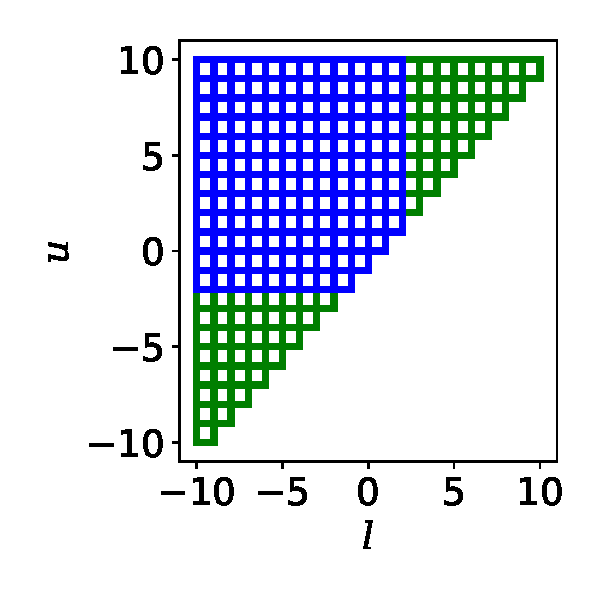
\includegraphics[width=0.4\linewidth]{offlinesyn/figs/partition.pdf}
	\caption{Partition of $ I_x $ for the Swish activation function, where the blue boxes belong
	to $ I_{tan} $, and the green boxes belong to $ I_{2pt} $.
	\label{offlinesyn:fig:partition}}
%	\vspace{-3ex}
\end{figure}
%\end{wrapfigure}

\subsection{Partitioning the Input Interval Space ($I_x$)}

A key consideration when partitioning $ I_x $ is how to represent each disjoint
subset of input intervals. While we could use a highly expressive representation such as polytope
or even use non-linear constraints, for efficiency reasons, we represent each
subset (of input intervals) as a box. Since a subset uses either the two-point
form template or the tangent-line form template, the input interval space can
be divided into
$I_x = I_{2pt}\cup I_{tan}$.
%
Each of $I_{2pt} $ and $ I_{tan} $ is  a set of boxes.


At a high-level, our
approach first partitions $ I_x $ into uniformly sized disjoint boxes, and then
assigns each box to either $ I_{2pt} $ or $ I_{tan} $. In
Figure~\ref{offlinesyn:fig:partition}, we illustrate the partition computed for $
swish(x)
= x \cdot sigmoid(x) $. The $x$-axis and $y$-axis represent the lower bound $ l
$ and
the upper bound $ u $, respectively, and thus a point $ (l, u) $ on this graph
represents the interval $ [l, u] $, and a box on this graph denotes  the set
of intervals represented by the points contained within it. We give details on
computing the partition below.

\paragraph{Defining the Boxes}

We first define a constant parameter $ c_s $, which is the width and height
of each box in the partition of $ I_x $. In Figure~\ref{offlinesyn:fig:partition},
$ c_s =
1 $. The benefits of using a smaller $ c_s $ value is two-fold. First, it allows
us to more accurately choose the proper template (two-point or tangent) for a
given interval $ [l, u] $. Second, as mentioned previously, the negative impact
of a template with a large violation (i.e., large $ \epsilon $) is localized to
a smaller set of input intervals.

Assuming that $ (u_x - l_x) $ can be divided by $c_s$, then we have $
(\frac{u_x -l_x}{c_s})^2 $ disjoint boxes in the partition of $ I_x $, which we
represent by $ I_{i,j} $ where $ i,j \in \{1..\frac{u_x - l_x}{c_s}\} $.
%
$ I_{i,j} $ represents the box whose lower-left corner is located at $ (l_x + i
\cdot c_s, l_x + j \cdot c_s) $, or
%
alternatively we have $ I_{i, j} = \{ [l,u] \mid l\in [l_x + i \cdot c_s, l_x +
i \cdot c_s + c_s], u \in [l_x + j \cdot c_s, l_x + j \cdot c_s + c_s]\}$.


To determine which boxes $ I_{i,j} $ belong to the subset $ I_{2pt} $, we
uniformly sample intervals $ [l, u] \in I_{i,j} $. Then, for each sampled
interval $ [l, u] $, we compute the two-point form for $ [l, u] $, and attempt
to search for a counter-example to the equation $ \sigma(x) \leq
\mathcal{G}_{a_u}(l, u)x + \mathcal{G}_{b_u}(l, u) $ by sampling $ x
\in [l, u] $.
%
If a counter-example is not found for more than half of the
sampled $ [l, u] \in I_{i,j} $, we add the box $ I_{i, j} $ to $ I_{2pt} $,
otherwise we add the box to $ I_{tan} $.

We note that more sophisticated (probably more expensive) strategies for
assigning templates exist. We use this strategy simply because it is efficient.
We also note that some boxes in the partition may contain invalid intervals
(i.e., we have $ [l, u] \in I_{i,j} $ where $ u < l $). These invalid intervals
are filtered out during the final verification step  described in
Section~\ref{offlinesyn:sec:soundness}, and thus do not affect the soundness of our
algorithm.

\subsection{Learning the Function $ g(l, u) $}\label{offlinesyn:sec:learning}

In this step, for each box $ I_{i,j} \in I_{tan} $, we want to learn a
function $ g(l, u) = t $ that returns the tangent point for any given
interval $[l,u] \in I_{i,j}$, where $ t $ will be used to compute the
tangent-line form upper bound as defined in
Equation~\ref{offlinesyn:eq:template-tan}.
%
This process is done for all boxes in $ I_{tan} $,
resulting in a separate $ g(l, u) $ for each box $ I_{i,j} $.
%
A sub-goal when learning $
g(l, u) $ is to maximize the tightness of the resulting upper bound, which in
our case means minimizing the volume below the tangent line.

We leverage machine learning techniques (specifically linear regression
or a small neural network with ReLU activation) to learn $ g(l, u) $, which means we need a
procedure to generate training examples. The examples must have the form $ ((l,
u), t) $. To generate the training examples, we
(uniformly) sample $ [l, u] \in I_{i,j} $, and for each sampled $ [l, u] $, we
attempt to find a tangent point $ t $ whose tangent line represents a tight
upper bound of
$\sigma(x)$. Then, given the training examples, we use standard machine
learning techniques to learn $ g(l, u) $.

The crux of our approach is generating the training examples. To generate a
single example for a fixed $ [l, u] $, we follows two steps: (1) generate
upper bound coefficients $ a_u, b_u $, and then (2) find a tangent point
$ t $ whose tangent line is close to $ a_u, b_u $. In the following paragraphs, we
describe the process for a fixed $ [l, u] $, and then discuss the machine
learning procedure.

%\begin{wrapfigure}{R}{0.5\textwidth}
\begin{figure}[t]
	\centering
	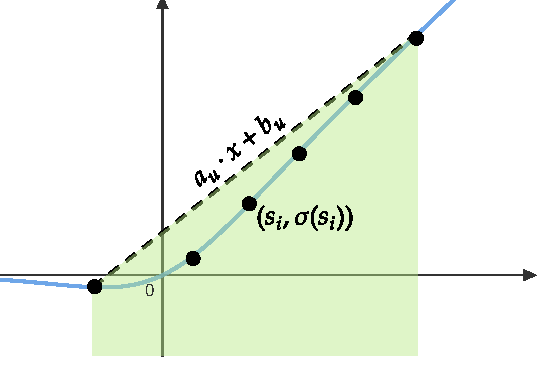
\includegraphics[width=0.5\linewidth]{offlinesyn/figs/sampling-lp.pdf}
	\caption{Illustration of the sampling and linear programming procedure for
	computing an upper bound. Shaded green region illustrates the volume below
	the upper bound.\label{offlinesyn:fig:samplelp}}
\end{figure}
%\end{wrapfigure}

\subsubsection{Generating Example Coefficients $ a_u, b_u $}
Given a fixed $ [l, u] $, we aim to generate upper bound coefficients $ a_u,
b_u $. A good generation procedure has three criteria: (1) the coefficients
should be tight for the input interval $ [l, u] $, (2) the coefficients should
be sound, and (3)
the generation should be fast. The first two criteria are intuitive: good training examples
will result in a good learned model. The third is to ensure that we can
generate a large number of examples in a reasonable amount of time.
Unfortunately, the second and third criteria are at odds, because proving
soundness is inherently expensive. To ensure a reasonable runtime, we relax the
second criteria to \textit{probably} sound. Thus our final goal is to minimize
volume below $ a_u, b_u $ such that $ \sigma(x) \leq a_u\cdot x + b_u $
\textit{probably} holds for $ x \in [l, u] $.

Our approach is inspired by a prior
work~\cite{ryou2021scalable,balunovic2019certifying}, which formulates the goal of a non-linear optimization problem
as a linear program that can be solved efficiently. Our approach samples points
$ (s_i, \sigma(s_i)) $ on the activation function for  $ s_i \in [l, u] $,
which are used to to convert the nonlinear constraint $ \sigma(x) \leq a_u\cdot
x + b_u $ into a linear one, and then uses volume as the objective (which is
linear). For a set $ S $ of sample points $ s_i \in [l, u] $, the
linear program we solve is:
\begin{gather*}
	\mathrm{minimize:} \; \mathrm{volume \;below}\;\; a_u\cdot x + b_u \\
	\mathrm{subj.\; to:} \;\; \bigwedge_{s_i \in S}
	\sigma(s_i) \leq a_u\cdot s_i + b_u
\end{gather*}
We illustrate this in Figure~\ref{offlinesyn:fig:samplelp}.
Solving the above problem results in $ a_u, b_u $, and the prior
work~\cite{ryou2021scalable,balunovic2019certifying} proved that the solution
(theoretically) approaches the optimal and sound $ a_u, b_u $ as the number of
samples goes to infinity. We use Gurobi~\cite{gurobi} to solve the linear
program.

\subsubsection{Converting $ a_u, b_u $ to a Tangent Line}
To use the generated $ a_u, b_u $ in the tangent-line form template,
we must find a point $ t $ whose tangent line is close to $ a_u, b_u $.
That is, we require that the following condition (almost) holds:
\begin{gather*}
	(\sigma'(t) = a_u) \wedge (\sigma'(t)\cdot t + \sigma(t) = b_u)
\end{gather*}
To solve the above problem, we use local optimization techniques (specifically a
modified Powell's method~\cite{powell1964efficient} implemented in
SciPy~\cite{2020SciPy-NMeth}, but most common techniques would work) to find a
solution to $ \sigma'(t) = a_u $.


We then check that the right side of the above formula almost holds
(specifically, we check ($ |(\sigma'(t)\cdot t + \sigma(t)) - b_u
| \leq 0.01 $). If the local optimization does not converge (i.e., it
does not find a $ t $ such that $ \sigma'(t) = a_u $), or the check on
$ b_u $ fails, we throw away the example and do not use it in
training.
\begin{figure}[t]
	\centering
	\begin{minipage}{.48\linewidth}
		\centering
		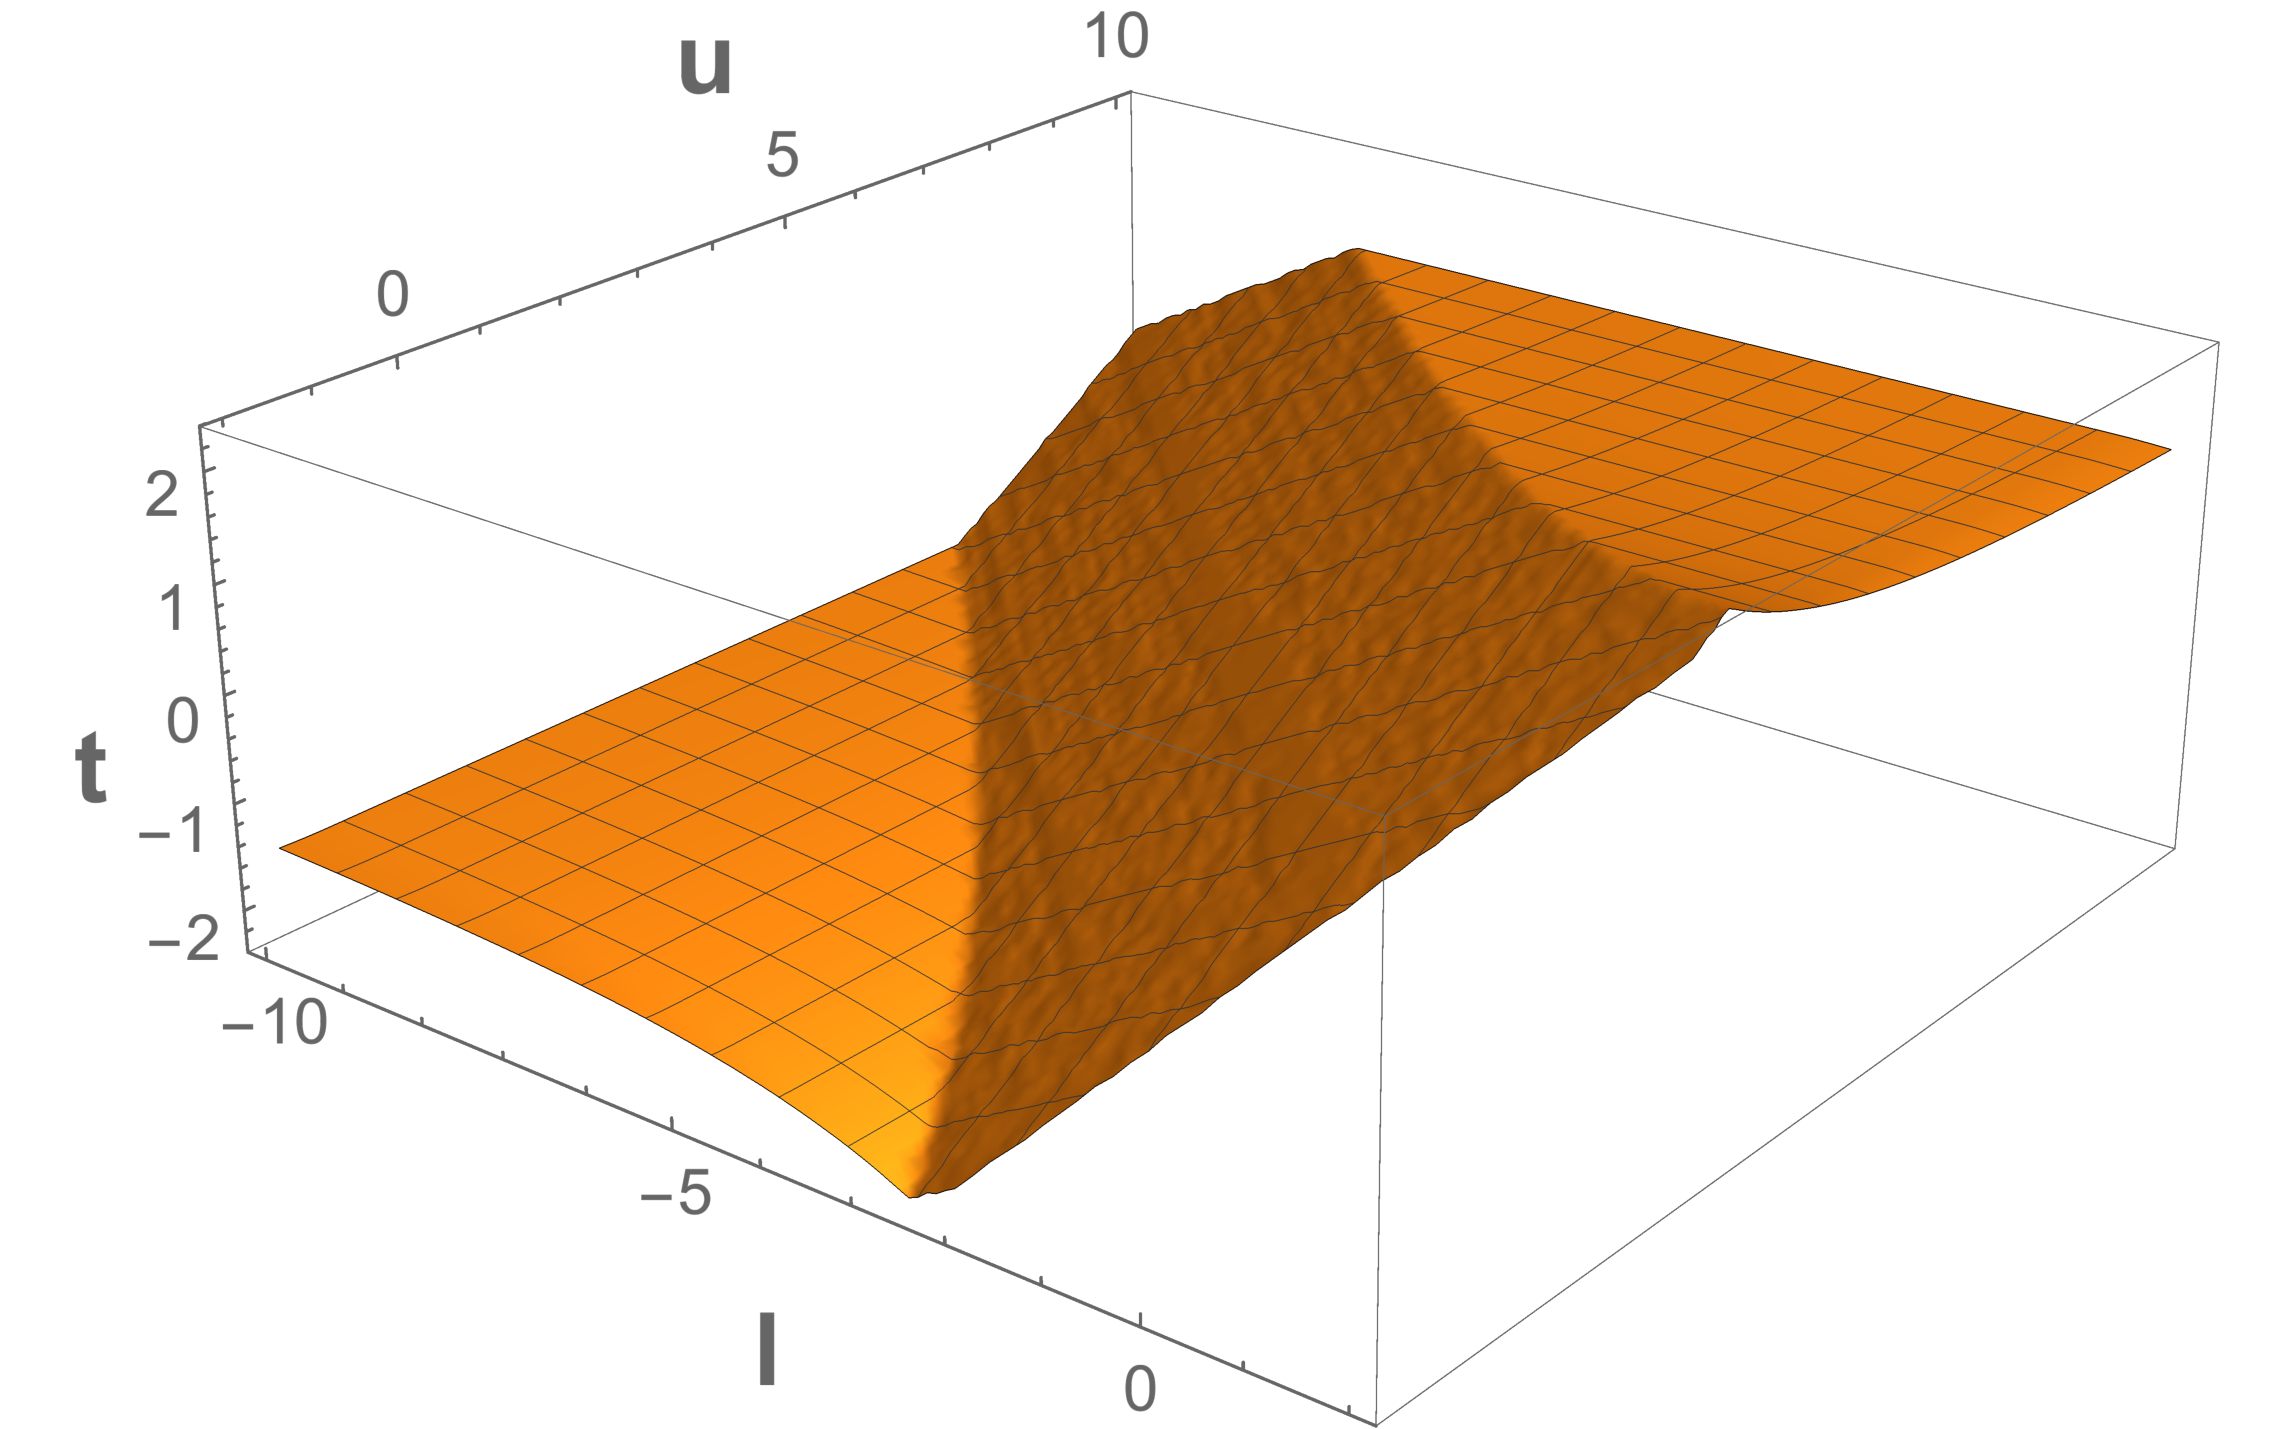
\includegraphics[width=\linewidth]{offlinesyn/figs/tanplot.pdf}
	\end{minipage}\hspace{12pt}%
	\begin{minipage}{.48\linewidth}
		\centering
		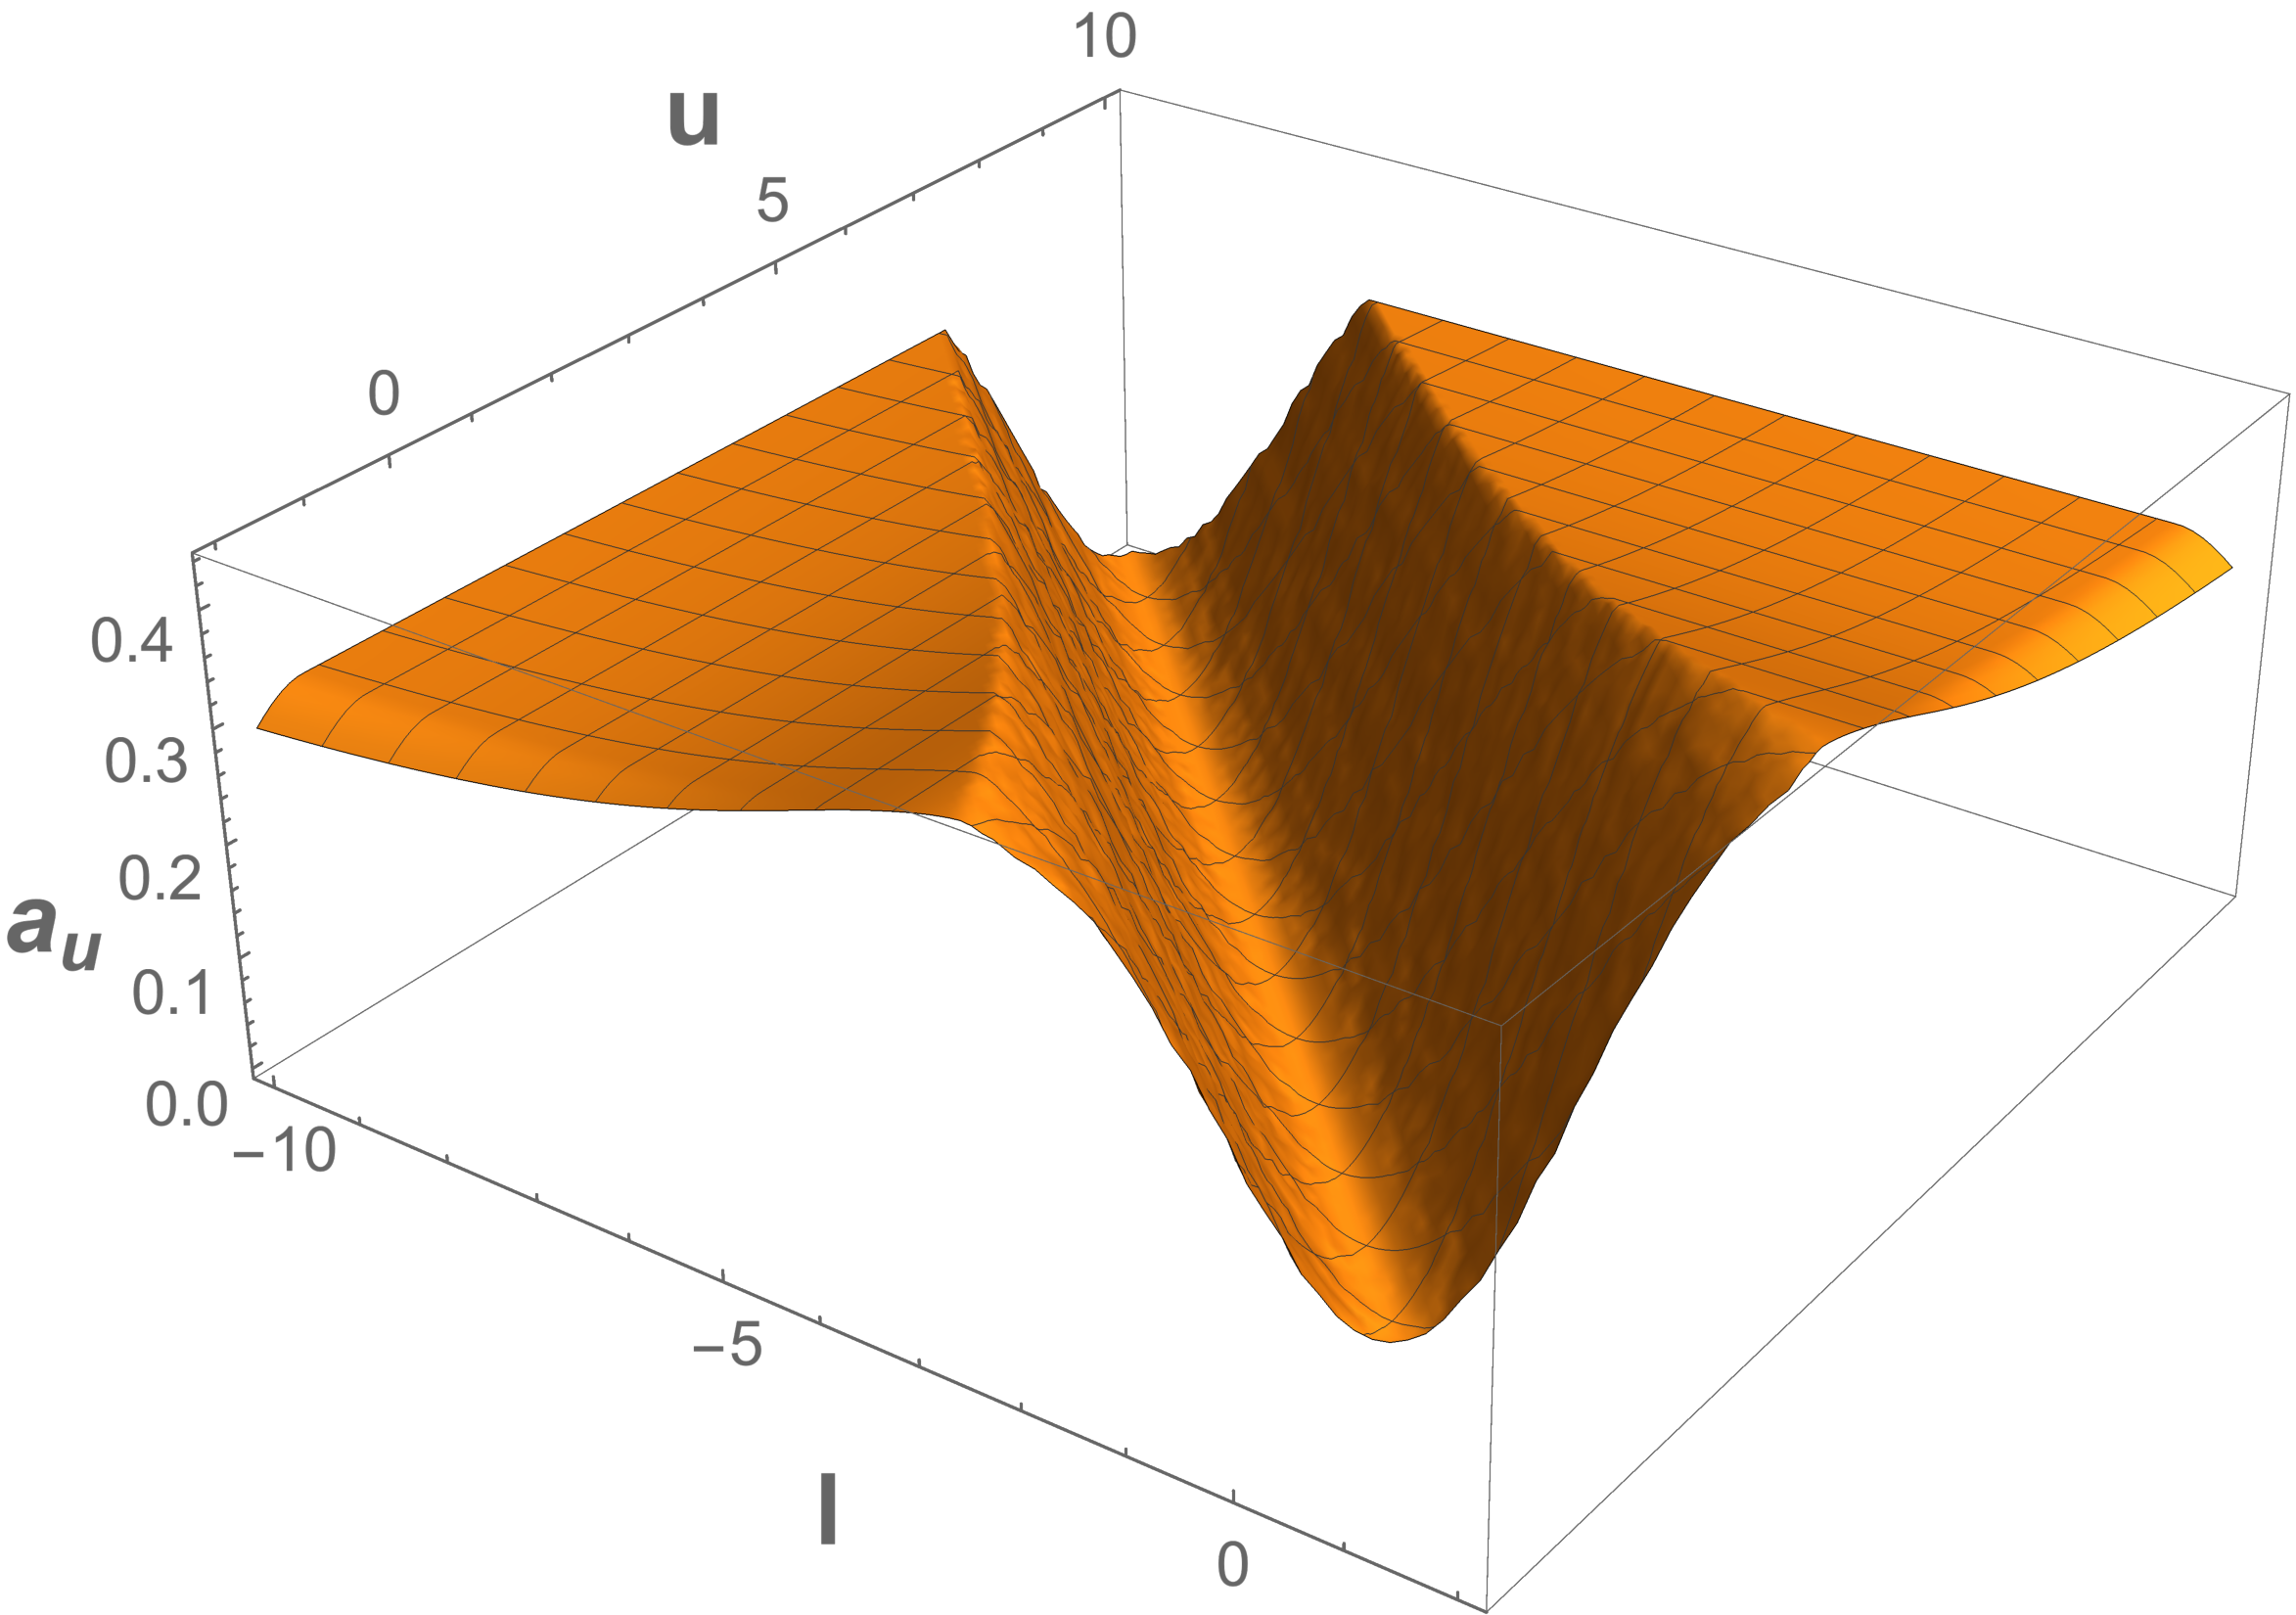
\includegraphics[width=\linewidth]{offlinesyn/figs/aplot.pdf}
	\end{minipage}
	\caption{Plots of the training examples, smoothed with linear
	interpolation. On the left: a plot of $ ((l, u), (t)) $, and on the right:
	a plot of $ ((l, u), (a_u)). $\label{offlinesyn:fig:targetfunc}}
	\label{offlinesyn:fig:funcstolearn}
\end{figure}

One may ask the question: could we simply train a model to directly predict the
coefficients $ a_u $ and $ b_u $, instead of predicting a tangent point and
then converting it to the tangent line? The answer is yes, however this
approach has two caveats. The first caveat is that we will lose the inherent
tightness that we gain with the tangent-line form -- we no longer have a
guarantee that the computed linear bound will touch $ \sigma(x) $ at
any point. The second caveat is  that the relationship between $ l, u $ and $ t $
tends to be close to linear, and thus easier to learn, whereas the relationship
between $ l, u$ and  $a_u $, or between $ l, u$ and $ b_u $,  is highly nonlinear.
We illustrate these
relationships as plots in Figure~\ref{offlinesyn:fig:targetfunc}. The left graph
plots the
generated training examples $ ((l, u), t) $, converted to a smooth function
using linear interpolation. We can see most regions are linear, as shown by the
flat sections. The right plot shows $ ((l, u), a_u) $, where we can see
the center region is highly nonlinear.

\subsubsection{Training on the Examples}
% TODO: Need ALGORITHMS!!!!!
Using the procedure presented so far, we sample $ [l, u] $ uniformly from $
I_{i,j} $ and generate the corresponding $ t $ for each of them. This results
in a training dataset of $ r $ examples $ \mathcal{D}_{train} = \{ ((l_i, u_i),
t_i) ~|~ i \in \{1..r\} \} $. We then choose between one of two models -- a
linear regression model or a 2-layer, 50-hidden-neuron, ReLU network -- to become
the final function $ g(l, u) $. To decide, we train both model types, and choose the one
with the lowest error, where error is measured as the mean absolute error. We give
details below.

A linear regression model is a function $ g(l, u) = c_1 \cdot l +
c_2 \cdot u + c_3 $, where $ c_i \in \mathbb{R} $ are coefficients
learned by minimizing the \textit{squared error}, which formally is:
\begin{equation}\label{offlinesyn:eq:sqerror}
	\sum_{((l_i, u_i), t_i) \in D_{train}} (g(l_i, u_i) - t_i)^2
\end{equation}
Finding the coefficients $ c_i $ that minimize the above constraint has a closed-form
solution, thus convergence is guaranteed and optimal, which is desirable.

However, sometimes the relationship between $ (l, u) $ and $ t $ is nonlinear,
and thus using a linear regression model may result in a poor-performing $ g(l,
u) $, even though the solution is optimal. To capture more complex
relationships, we also consider a 2-layer ReLU network where $
\mathbf{W}_0 \in \mathbb{R}^{2\times50} $, $ \mathbf{W}_1 \in
\mathbb{R}^{50\times1} $, $ \mathbf{b}_0 \in \mathbb{R}^{50} $, $ \mathbf{b}_1
\in \mathbb{R} $, and we have $ g(l, u) = \text{ReLU}(\langle l,u \rangle^T
\cdot \mathbf{W}_0 + \mathbf{b}_0) \cdot \mathbf{W}_1 + \mathbf{b}_1 $. The
weights and biases are initialized randomly, and then we minimize the
squared error (Equation~\ref{offlinesyn:eq:sqerror}) using gradient
descent. While convergence to the optimal weights is not guaranteed in
theory, we find in practice it usually converges.

We choose these two models because they can capture a diverse set of $ g(l , u) $ functions. While
we could use other prediction models, such as polynomial regression, generally, a neural
network will be equally (if not more) expressive. However, we believe exploring
other model types or architectures of neural networks would be an interesting
direction to explore.

%\textcolor{red}{Need to explain, in more detail,  how ``vanilla machine
%learning models'' are actually used.  I am sure people what to know more about
%this -- merely saying vanilla machine learning model is not good enough.  For
%example, was it a linear regression, or a low-degree polynomial regression,
%and
%what does the neural network look like, and what ``small'' really means?}


\subsection{Ensuring Soundness of the Linear
Approximations}\label{offlinesyn:sec:soundness}
For a given $ I_{i, j} $, we must ensure that its corresponding coefficient
generator functions $ \mathcal{G}_{a_u}(l ,u)$ and $ \mathcal{G}_{b_u}(l ,u) $
are sound, or in other
words, that the following condition does \textbf{not} hold:
\begin{gather*}\label{offlinesyn:eq:sound-opt}
\exists [l, u] \in I_{i, j}, \; x \in [l, u] ~.~
\sigma(x) > \mathcal{G}_{a_u}(l, u)\cdot x + \mathcal{G}_{b_u}(l, u)
\end{gather*}
We ensure the above condition does not hold (the formula is unsatisfiable) by bounding the \textit{maximum violation} on
the clause $ \sigma(x) > \mathcal{G}_{a_u}(l, u)\cdot x + \mathcal{G}_{b_u}(l,
u) $,
which we formally define as
$ \Delta(l, u, x) =  \sigma(x) - (\mathcal{G}_{a_u}(l, u)\cdot x +
\mathcal{G}_{b_u}(l, u)) $. $ \Delta $ is
positive when the previous clause holds.  Thus, if we can compute an upper bound
$ \Delta_u $, we can set the $ \epsilon $ term in $ \mathcal{G}_{b_u}(l, u) $
to $ \Delta_u $
to ensure the clause does not hold, thus making the coefficient generator functions sound.

To compute $ \Delta_u $, we solve (i.e., bound) the following optimization
problem:
\begin{gather*}\label{offlinesyn:eq:opt}
\mathrm{for:}\;\; l, u, x \in [l_{i,j}, u_{i,j}] \\
\mathrm{maximize:}\;\; \Delta(l, u, x)\\
\mathrm{subj. \; to:}\;\;
l < u \wedge l \leq x \wedge x \leq u
\end{gather*}
where $ l_{i,j}, u_{i,j} $ are the minimum lower bound and maximum upper bound,
respectively, for any interval in $ I_{i, j} $.
The above problem can be solved using the general framework of interval
analysis~\cite{moore2009introduction} and branch-and-prune
algorithms~\cite{benhamou2006continuous}.

Letting
$ \Delta_{search} = \{(l, u, x) | l, u, x \in [l_{i,j}, u_{i,j}] \} $
be the domain over which we want to bound $ \Delta $,
we can bound $ \Delta $ over $ \Delta_{search} $ using interval analysis.
%
In
addition, we can improve the bound in two ways: \textit{branching} (i.e.,
partitioning $ \Delta_{search} $ and bounding $ \Delta $ on each subset
separately) and \textit{pruning} (i.e., removing from $ \Delta_{search} $
values that violate the constraints $ l < u \wedge l \leq x \wedge x \leq u $).
The tool IbexOpt~\cite{chabert2009contractor} implements such an algorithm, and
we use it solve the above optimization problem.

One practical consideration when solving the above optimization problem is the
presence of division by zero error. In the two-point template, we have
$ \mathcal{G}_{a_u}(l, u) = \frac{\sigma(u) - \sigma(l)}{u - l} $. While we
have the
constraint $ l < u $, from an interval analysis perspective, $
\mathcal{G}_{a_u}(l, u) $ goes
to infinity as $ u - l $ goes to 0, and indeed, if we gave the above problem to
IbexOpt, it would report that $ \Delta $ is unbounded. To account for this, we
enforce a minimum interval width of $ 0.01 $ by changing $ l < u $ to $ 0.01 <
u - l $.

%\begin{figure}[t]
%	\centering
%	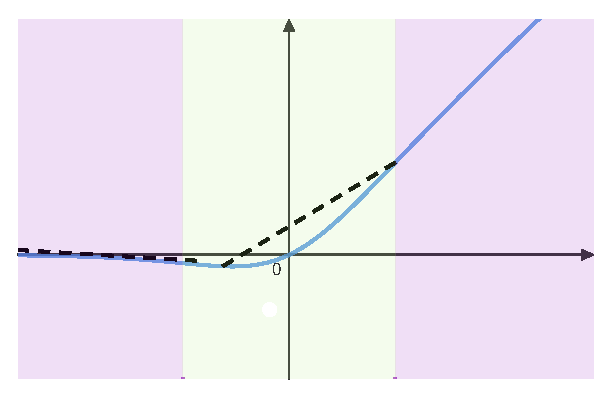
\includegraphics[width=0.5\linewidth]{offlinesyn/figs/convex.pdf}
%	\caption{An illustration of the convex (green) and concave (purple) regions
%	of Swish, and two linear upper bounds.\label{offlinesyn:fig:convex}}
%\end{figure}
%\subsubsection{Exploiting Convex and Concave Regions}
%Another advantage of structuring our templates as two-point and tangent-point
%templates is that they allow us to exploit the convex ($ \cup $-shaped) and
%concave ($ \cap $-shaped) regions of $ \sigma(x) $. Formally, we denote by $
%[l_i^\cup, u_i^\cup] $ an interval over which $ \sigma(x) $ is convex (there
%may be several, hence the $ i $), and $ [l_i^\cap, u_i^\cap] $ a concave
%region. We defer discussing how to obtain these intervals until the end of this
%subsection. In Figure~\ref{offlinesyn:fig:convex}, we illustrate the convex and
%concave
%regions of Swish.
%
%For the two-point template, we can exploit the convex regions. For a convex
%interval $ [l_i^\cup, u_i^\cup] $, the two-point form for any interval $ [l, u]
%\subseteq [l_i^\cup, u_i^\cup] $ is guaranteed to be a sound
%upper bound (this follows from the definition of convexity). We illustrate such
%a two-point form bound in Figure~\ref{offlinesyn:fig:convex} in the shaded green
%region.
%We can exploit this to skip verification for some two-point form $ I_{i, j} $.
%Formally, let $ I_\cup = \bigcup_i [l_i^\cup, u_i^\cup] \times [l_i^\cup,
%u_i^\cup] $ be the set of all intervals contained in a convex region. If we
%have $ I_{i, j} \ I_\cup = \emptyset $, then we can skip the verification of $
%I_{i,j} $'s template all together (i.e. set $ \epsilon = 0 $).
%
%In addition, we can exploit concave regions to partially or
%completely verify a tangent-point template. Concave regions have the following
%property: given a concave interval $ [l_i^\cap, u_i^\cap] $,
%a line tangent to $ \sigma(x) $ at point $ t \in [l_i^\cap, u_i^\cap] $ must
%be entirely above $ \sigma(x) $ over the interval $ [l_i^\cap, u_i^\cap] $
%(this follows the from the definition of concavity). We illustrate such a
%tangent line in the shaded purple region in Figure~\ref{offlinesyn:fig:convex}.
%To verify
%soundness of this tangent line, we would only need to look for violations
%outside the purple shaded region.
%
%However, we cannot directly exploit concavity without modifying our
%tangent-point template. In order to exploit it, we must ensure that, for some
%fixed concave region $ [l_i^\cap, u_i^\cap] $, $  g(l, u) \in [l_i^\cap,
%u_i^\cap] $ for all $ [l, u] \in I_{i,j} $. If we can ensure this, then we
%modify the domain of the variable $ x $ in the optimization problem in
%Equation~\ref{offlinesyn:eq:opt} to be $ x \in [l_{i,j}, u_{i,j}] \ [l_i^\cap,
%u_i^\cap] $ because there cannot be any violations of
%Equation~\ref{offlinesyn:eq:sound-opt} for $ x \in [l_i^\cap, u_i^\cap] $. This
%reduction
%in domain greatly speeds up solving Equation~\ref{offlinesyn:eq:opt}.
%
%To choose the appropriate $ [l_i^\cap, u_i^\cap] $ for a given $ I_{i, j} $, we
%use the training examples $ D_{train} $ described in
%Section~\ref{offlinesyn:sec:learning}.
%
%
%\textit{Finding Convex/Concave Intervals}
%We take a very simple sampling approach for finding the convex and concave
%intervals, and we omit a full discussion. At a high-level, we sample points on
%the second derivative $ \sigma''(x) $ to find intervals where it is always
%positive and always negative. We then verify that these intervals are indeed
%convex/concave by using Ibex~\cite{chabert2009contractor} to prove $ \forall x
%\in [l_i^\cup, u_i^\cup] ~.~ \sigma''(x) > 0 $.

%\subsubsection{Verifying the Two-Point Form Bounds}
%
%In this step, we are given $ I_{2pt} $, which is simply a list of $ n_{2pt} $
%boxes that we refer to simply as $ I_{k} $ for $ k \in \{1..n_{2pt}\} $. For
%each $ I_k $, we must verify:
%% TODO: put the proper bound on x
%\begin{gather*}
%\forall x, (l, u) \in I_k \\
%l \geq u \vee l > x \vee x > u \; \vee \\
%\sigma(x) \leq a_u(l, u)x + b_u(l, u)
%\end{gather*}
%
%% removing intervals that are entirely convex in a convex region
%Let $ I_\smile $ be the set of all intervals that are entirely contained in a
%convex region. We only need to verify the portion of $ I_k $ not in $ I_\smile
%$, i.e., $ I_k - I_\smile $.
%
%% optimizing verification of intervals that cross a
%
%\subsubsection{Verifying the Tangent Line Form Bounds}
%
%We restrict $ g(l, u) $ so that it is always in a concave region $ [ l_\frown,
%u_\frown ] $, so we can always prune the concave region from the search space.

\subsection{Efficient Lookup of the Linear Bounds}

Due to partitioning $ I_x $, we must have a procedure for looking up the
appropriate template instance for a given $ [l, u] $ at the application time.
Formally, we need to find the box
$ I_{i, j} $, which we denote $ [l_l, u_l] \times [l_u, u_u] $,
such that $ l \in [l_l, u_l] $ and $ u \in [l_u, u_u] $, and retrieve the
corresponding template. Lookup can actually present a significant runtime overhead if
not done with care. One approach is to use a data structure similar to an interval
tree or a quadtree~\cite{finkel1974quad}, the latter of which has $
\mathcal{O}(log(n)) $ complexity. While the quadtree would be the most
efficient for an arbitrary partition of $ I_x $ into boxes, we can in fact
obtain $ \mathcal{O}(1) $ lookup for our partition strategy.

We first note that each box, $ I_{i, j} $,
can be uniquely identified by $ l_l $ and $ u_u $. The point $ (l_l, u_u) $
corresponds to the top-left corner of a box in
Figure~\ref{offlinesyn:fig:partition}.
%
Thus we build a lookup dictionary keyed by $ (l_l, u_u) $ for each box that
maps to the corresponding linear bound template.
%
To perform lookup, we exploit the structure of the partition: specifically,
each box in the partition is aligned to a multiple of $ c_s $.
%
Thus, to lookup $ I_{i,j} $ for a given $ [l, u] $, we view $ (l, u) $ as a
point on the graph of Figure~\ref{offlinesyn:fig:partition}, and the lookup
corresponds to
moving left-ward and upward from the point $ (l, u) $ to the nearest upper-left
corner of a box.
%
More formally, we perform lookup by rounding $ l $ down to the nearest
multiple of $ c_s $, and $ u $ upward to the nearest multiple of $ c_s $.
The top-left corner can then be used to lookup the appropriate template.


%\begin{itemize}
%	\item min width to ensure efficiency of bounding max viol of two point form
%	(there could be a zero denom if we don't have a min width)
%	\item what if we encounter $ [l, u] $ at runtime that is out of the $ l_x,
%	u_x $ range? we fall back to IBP
%	\item efficient lookup
%\end{itemize}

\section{Evaluation}
\label{offlinesyn:sec:experiment}

We have implemented our approach as a software tool that synthesizes a linear
bound generator function $ \mathcal{G}(l,u) $ for any given activation function
$ \sigma(x) $ in the input universe $ x \in
[l_x, u_x] $. The output is a function that takes as input $ [l, u] $ and
returns
coefficients $ a_l, b_l, a_u, b_u $ as output. For all experiments, we use $ l_x = -10,
u_x = 10 $, $ c_s = 0.25 $, and a minimum interval width of $ 0.01 $.
%
After the generator function is synthesized, we integrate it into
\autolipra{}, a state-of-the-art neural network verification tool, which allows us to analyze neural networks
with $ \sigma(x) $ as activation functions.

\subsection{Benchmarks}


\subsubsection{Neural Networks and Datasets}
Our benchmarks are eight deep neural networks trained on the following two
datasets.

\textit{MNIST}. MNIST~\cite{LecunBBH98} is a set of images of hand-written
digits
each of which are labeled with the corresponding written digit. The images are
28x28 grayscale images with one of ten written digits. We use a convolutional
network architecture with 1568, 784, and 256 neurons in its first, second, and
third layer, respectively. We train a model for each of the activation
functions described below.

\textit{CIFAR}. CIFAR~\cite{krizhevsky2009learning} is a set of images
depicting one of 10
objects (a dog, a truck, etc.), which are hand labeled with the
corresponding object. The images are 32x32 pixel RGB images. We use a
convolutional architecture with 2048, 2048, 1024, and 256 neurons in the first,
second, third, and fourth layers, respectively. We train a model for each of
the activation functions described below.

\subsubsection{Activation Functions}
Our neural networks use one of the activation functions shown
Figure~\ref{offlinesyn:fig:acts} and defined in Table~\ref{offlinesyn:tbl:acts}.
They are
Swish~\cite{hendrycks2016gaussian,ramachandran2017searching},
GELU~\cite{hendrycks2016gaussian}, Mish~\cite{misra2019mish},
LiSHT~\cite{roy2019lisht}, and AtanSq~\cite{ramachandran2017searching}. The
first two are used in language models such as
GPT~\cite{radford2018improving}, and have been shown to achieve
the best performance for some image classification
tasks~\cite{ramachandran2017searching}. The third and fourth two are variants
of the first two, which are shown to have desirable theoretical properties. The
last was discovered using automatic search
techniques~\cite{ramachandran2017searching}, and found to perform on par with
the state-of-the-art. We chose these activations because they are representative of
recent developments in deep learning research.

\begin{figure}[t]
	\centering
	\begin{minipage}{.48\textwidth}
		\centering
		\begin{table}[H]
			\caption{Definitions of activation functions used in our experiments.}
			\scalebox{0.86}{%
				\renewcommand{\arraystretch}{1.2}
				\begin{tabular}{|l|l|}
					\hline
					Name  &
					Definition
					\\
					\hline
					Swish & $x \cdot
					sigmoid(x)$                                              \\
					\hline
					GELU  & $ 0.5 x ( 1 + \tanh{[ \sqrt{2 / \pi } (x + 0.044715x
						^{3} ) ] } )$ \\ \hline
					Mish  & $x \cdot \tanh{[\text{ln}( 1 + e^x
						)]}$                                    \\ \hline
					LiSHT & $x \cdot
					\tanh{(x)}$
					\\
					\hline
					AtanSq & $ (\text{tan}^{-1}(x))^2  - x $ \\ \hline
				\end{tabular}}
			\label{offlinesyn:tbl:acts}
		\end{table}
	\end{minipage}\hspace{12pt}%
	\begin{minipage}{.48\textwidth}
		\centering
		\scalebox{1.1}{
			\begin{tikzpicture}
        \begin{axis}[
            xmin = -5, xmax = 3,
            ymin = -1.2, ymax = 3.5,
            xtick distance = 10,
            ytick distance = 10,
            %grid = both,
            %minor tick num = 1,
            %major grid style = {lightgray},
            %minor grid style = {lightgray!25},
            width = \linewidth,
            height = 0.75\linewidth,
            xticklabel=\empty,yticklabel=\empty,
            minor tick num=0,
%            major tick num=0,
%            hide axis,
            axis lines = middle,
            legend cell align = {left},
%            legend pos = north west,
			set layers=standard,
	        legend to name=grouplegend,
	        legend entries={{Swish},
	        	{LiSHT},
	        	{Mish},
	        	{GELU},
        		{AtanSq},},
        	legend style={nodes={scale=0.9, transform shape},font=\scriptsize,
        	draw=none,fill=white,align=left},
        ]
			\addplot[actfunc, blue] {x * (1 / (1 + exp(-x)))};
            \addplot[actfunc, green,domain=-3:3] {x * tanh(x)};
            \addplot[actfunc, purple] {x * tanh(ln(1+exp(x)))};
            \addplot[actfunc, cyan] {0.5*x * ( 1 + tanh(sqrt(2/pi) * (x+
            0.044715 * (x ^3) ) ) )};
            \addplot[actfunc, purple, domain=-2:2.5] {rad(atan(x))^2 - x};
			\coordinate (leg) at (rel axis cs:-0.15,0.95);

%            \legend{
%             {$ 0.5 x ( 1 + \tanh{ \sqrt{2 / \pi } (x + 0.044715 x ^{3} ) } ) $
%              \\ (GeLU)},
%             {$ min(1, max(x, -1)) $ (Hard Tanh)},
%             $ 1 - e^{-e^{x}} $ (Log-Log),
%    	     $ x * \sigma(x) $ (Swish),
%                }
        \end{axis}
        \node[anchor= north west] at
        (leg){\pgfplotslegendfromname{grouplegend}};
\end{tikzpicture}
}
		\caption{Activation functions used in our experiments.}
		\label{offlinesyn:fig:acts}
	\end{minipage}
\end{figure}

\subsubsection{Robustness Verification}
% TODO: $\epsilon$ is used already!
We evaluate our approach on \textit{robustness} verification problems. Given a
neural network $ f: \mathbb{X} \subseteq \mathbb{R}^n \to \mathbb{Y} \subseteq
\mathbb{R}^m $ and an input $ \mathbf{x} \in \mathbb{X} $, we verify robustness
by proving that making a small $ p $-bounded perturbation ($ p \in \mathbb{R}
$) to $ \mathbf{x} $ does not change the classification. Letting $
\mathbf{x}[i] \in \mathbb{R} $ be the $ i^{th} $ element in $ \mathbf{x} $, we
represent the set of all perturbations as $ X \in \mathbb{IR}^n $, where $ X =
\bigtimes_{i=1}^n [\mathbf{x}[i] - p, \mathbf{x}[i] + p] $. We then compute $ Y
\in \mathbb{IR}^m $ where $ Y = \bigtimes_{i=1}^m [l_i,
u_i] $, and, assuming the target class of $ \mathbf{x} $ is $ j $, where $ j \in
\{1..m\} $, we prove robustness by checking $ (l_j > u_i)$ for all $i \neq j$ and $i \in
\{1..m\} $.

For each network, we take 100 random test images, and following prior
work~\cite{GehrMDTCV18}, we filter out misclassified images. We then take
the remaining images, and create a robustness verification problem for each
one. Again following prior work, we use $ p = 8/255 $ for MNIST networks
and $ p = 1/255 $ for CIFAR networks.

\subsection{Experimental Results}

Our experiments were designed to answer the following question: How do our
synthesized linear approximations compare with other state-of-the-art,
hand-crafted linear approximation techniques on novel activation functions?
%
To the best of our
knowledge,~\autolipra{}~\cite{autolipra} is the only neural network
verification tool capable of handling the activation functions we considered here
using static, hand-crafted approximations.
%
We primarily focus on comparing the number of verification problems solved
%
and we caution against directly comparing the runtime of our approach
against~\autolipra{}, as the latter is highly engineered for parallel computation,
whereas our approach is not currently engineered to take advantage of parallel computation (although it
could be).
%
We conducted all experiments on an 8-core 2.7GHz processor with 32GB of RAM.
\footnotetext[1]{\autolipra{} does not have an approximation for $
	\text{tan}^{-1} $.}
%
%\textcolor{red}{We only have one result able (using synthesized bounds for
%verification). Is it possible to show some statistics about the synthesis
%part?
%For example, during synthesis, what's the percentage boxes in
%$|I_{2pt}|/|I_x|$
%vs.  $|I_{tan}|/|I_x|$? How many boxes use linear regression and how many use
%ReLU network to store the $g(l,u)$? How many boxes failed the soundness
%verification and thus needed to be shifted by $$?  And in general, how
%much time was spent on each step of the synthesis procedure?}


We present results on robustness verification problems in
Table~\ref{offlinesyn:tbl:1}.
The first column shows the dataset and architecture. The next two columns show
the percentage of the total number of verification problems solved (i.e.,
robustness proved) and the total runtime in seconds for~\autolipra{}. The next
two columns show the same statistics for our approach. The final column
compares the
output set sizes of~\autolipra{} and our approach. We first define $ |Y| $ as
the volume of the (hyper)box $ Y $. Then letting $ Y_{auto} $ and $ Y_{ours} $
be the output set computed by~\autolipra{} and our approach, respectively, $
\frac{|Y_{ours}|}{|Y_{auto}|} $ measures the reduction in output set size. In
general, $ |Y_{ours} | < | Y_{auto} | $ indicates our approach is better
because it implies that our approach has more accurately approximated the true
output set, and thus $ \frac{|Y_{ours}|}{|Y_{auto}|} < 1 $ indicates our
approach is more accurate.


\begin{table}[t]
	\centering
	\caption{Comparison of the verification results of our approach and \autolipra{}.}
	\label{offlinesyn:tbl:1}
	\scalebox{0.9}{
		\renewcommand{\arraystretch}{1.15}

		\begin{tabular}{|ll|cr|cr|c|}
			\hline
			& \multicolumn{1}{c|}{\multirow{2}{*}{Network Architecture}} &
			\multicolumn{2}{l|}{AutoLiPRA~\cite{autolipra}}               &
			\multicolumn{2}{l|}{Our Approach }                           &
			\multirow{2}{*}{\ \ $ \frac{|Y_{ours}|}{|Y_{auto}|}$\ \ } \\ \cline{3-6}
			& \multicolumn{1}{c|}{}                                      &
			\multicolumn{1}{c|}{\% certified} & time (s) &
			\multicolumn{1}{l|}{\% certified} & \multicolumn{1}{l|}{time (s)}
			&                                                   \\ \hline \hline
			\multicolumn{1}{|l|}{MNIST} & 4-Layer CNN with
			Swish                                     &
			\multicolumn{1}{c|}{0.34}         & 15       &
			\multicolumn{1}{c|}{0.74}         & 195                           &
			0.59                                              \\ \cline{2-7}
			\multicolumn{1}{|l|}{}      & 4-Layer CNN with
			Gelu                                      &
			\multicolumn{1}{c|}{0.01}         & 359      &
			\multicolumn{1}{c|}{0.70}          & 289                           &
			0.22                                              \\ \cline{2-7}
			\multicolumn{1}{|l|}{}      & 4-Layer CNN with
			Mish                                      &
			\multicolumn{1}{c|}{0.00}         & 50       &
			\multicolumn{1}{c|}{0.28}         & 236                           &
			0.29                                              \\ \cline{2-7}
			\multicolumn{1}{|l|}{}      & 4-Layer CNN with
			LiSHT                                     &
			\multicolumn{1}{c|}{0.00}          & 15       &
			\multicolumn{1}{c|}{0.11}          & 289                           &
			0.32                                              \\ \cline{2-7}
			\multicolumn{1}{|l|}{}      & 4-Layer CNN with
			AtanSq\footnotemark{}                                 &
			\multicolumn{1}{c|}{-}            & -        &
			\multicolumn{1}{c|}{0.16}         & 233                           &
			-                                                 \\ \hline \hline
			\multicolumn{1}{|l|}{CIFAR} & 5-Layer CNN with
			Swish                                     &
			\multicolumn{1}{c|}{0.03}         & 69       &
			\multicolumn{1}{c|}{0.35}         & 300                           &
			0.42                                              \\ \cline{2-7}
			\multicolumn{1}{|l|}{}      & 5-Layer CNN with
			Gelu                                      &
			\multicolumn{1}{c|}{0.00}         & 1,217    &
			\multicolumn{1}{c|}{0.29}          & 419                           &
			0.21                                              \\ \cline{2-7}
			\multicolumn{1}{|l|}{}      & 5-Layer CNN with
			Mish                                      &
			\multicolumn{1}{c|}{0.00}         & 202      &
			\multicolumn{1}{c|}{0.29}         & 363                           &
			0.17                                              \\ \cline{2-7}
			\multicolumn{1}{|l|}{}      & 5-Layer CNN with
			LiSHT                                     &
			\multicolumn{1}{c|}{0.00}         & 68       &
			\multicolumn{1}{c|}{0.00}          & 303                           &
			0.09                                              \\ \cline{2-7}
			\multicolumn{1}{|l|}{}      & 5-Layer CNN with
			AtanSq\footnotemark[1]{}                                    &
			\multicolumn{1}{c|}{-}            & -        &
			\multicolumn{1}{c|}{0.22}          & 347                           &
			-                                                 \\ \hline
		\end{tabular}
	}

\end{table}


We point out three trends in the results. First, our automatically synthesized
linear approximations always result in more verification problems solved. This
is because our approach synthesizes a linear approximation specifically for $
\sigma(x) $, which results in tighter bounds. Second,~\autolipra{} takes longer
on more complex activations such as GELU and Mish, which have more elementary
operations than Swish and LiSHT. This occurs because~\autolipra{} has more
linear approximations to compute (it must compute one for every elementary
operation before composing the results together). On the other hand, our
approach computes the linear approximation in one step, and thus does not have
the additional overhead for the more complex activation functions. Third, our
approach always computes a much smaller output set, in the range of 2-10X
smaller, which again is a reflection of the tighter linear bounds.
%\paragraph{Overall Comparison}

%\textcolor{red}{Need to say a few words about CIFAR -- LiSHT, for which our
%approach proved 0\% -- what's the reason for that?  Furthermore, is it
%possible
%that, although both methods proved 0\%,  our approach is still be better than
%\autolipra{} in some sense?}
\paragraph{Synthesis Results} We also report some key metrics about the
synthesis procedure. Results are shown in Table~\ref{offlinesyn:tbl:synth}. The
first
three columns show the total CPU time for the three steps in our synthesis procedure. We
note that all three steps can be heavily parallelized, thus the wall clock time
is roughly 1/8 the reported times on our 8-core machine. The final column shows
the percentage of boxes in the partition that were assigned a two-point
template (we can take the complement to get the percentage of tangent-line
templates).

%\begin{wrapfigure}{R}{0.5\textwidth}
\begin{table}[t]
	\centering
	\caption{Statistics of the synthesis step in our
	method.\label{offlinesyn:tbl:synth}}
	\scalebox{0.9}{
	\begin{tabular}{|l|r|r|r|c|}
		\hline
		Activation $\sigma(x)$ & \begin{tabular}[c]{@{}l@{}}Partition\ \ \ \\ Time
		(s)\end{tabular} & \begin{tabular}[c]{@{}l@{}}      Learning\ \ \ \ \ \\ Time
		(s)\end{tabular} & \begin{tabular}[c]{@{}l@{}}Verification\\ Time
		(s)\end{tabular} & \ \ \ \ $\frac{|I_{2pt}|}{|I_x|}$\ \ \ \  \\ \hline \hline
		Swish       &
		81                                                           &
		1,762                                                        &
		20,815                                                           &
		0.45                      \\ \hline
		GELU        &
		104                                                          &
		2,113                                                        &
		45,504                                                           &
		0.57                      \\ \hline
		Mish        &
		96                                                           &
		2,052                                                        &
		38,156                                                           &
		0.45                     \\ \hline
		LiSHT       &
		83                                                           &
		1,650                                                        &
		61,910                                                           &
		0.46                      \\ \hline
		AtanSq      &
		85                                                           &
		1,701                                                        &
		18,251                                                           &
		0.38                      \\ \hline
	\end{tabular}
}
\end{table}
%\end{wrapfigure}

\section{Related Work}
\label{offlinesyn:sec:related}

Most closely related to our work are those that leverage
interval-bounding techniques to conduct neural network verification.
Seminal works in this area can
either be thought of as explicit linear bounding, or linear bounding
with some type of restriction (usually for efficiency). Among the explicit
linear bounding techniques are the ones used in
~\DeepPoly{}~\cite{SinghGPV19},~\autolipra{}~\cite{autolipra},
~\Neurify{}~\cite{WangPWYJ18nips}, and
similar
tools~\cite{balunovic2019certifying,du2021cert,ko2019popqorn,zhang2018efficient,WengZCSHDBD18,wu2021tightening,ryou2021scalable,shi2020robustness}.
On the other hand,  techniques using Zonotopes~\cite{GehrMDTCV18,MirmanGV18} and
symbolic intervals~\cite{WangPWYJ18} can be thought of as restricted linear
bounding. Such approaches have an advantage in scalability, although they
may sacrifice completeness and accuracy. In addition, recent work leverages
semi-definite approximations~\cite{hu2020reach}, which allow for more
expressive, nonlinear lower and upper bounds. In addition, linear
approximations are used in nonlinear programming and
optimization~\cite{chabert2009contractor,trombettoni2011inner}.
However, to the best of our
knowledge, none of these prior works attempt to automate the process of crafting
the bound generator function $\mathcal{G}(l, u) $.


Less closely related are neural network verification approaches based
on solving systems of linear
constraints~\cite{KatzBDJK17,KatzHIJLLSTWZDK19,Ehlers17,HuangKWW17,BastaniILVNC16,HuangKWW17,baluta2019quantitative,tjeng2019evaluating}.
Such approaches typically only apply to networks with piece-wise-linear
activations such as ReLU and max pooling, for which there is little need to
automate any part of the verification algorithm's design (at least with respect
to the activation functions). They do not handle novel activation functions such as the ones concerned in our work.  These approaches have the advantage of being
complete, although they tend to be less scalable than interval analysis based
approaches.


Finally, we note that there are many works built off the initial linear approximation
approaches, thus highlighting the importance of designing tight and sound linear
approximations in general~\cite{Singh2019krelu,SinghGPV19iclr,WangPWYJ18nips,tran2019star,tran2020verification}.


%\paragraph{Future Work} An interesting line of future work would be
%to automatically synthesize other types of approximations, such as zonotopes
%or semi-definite
%relaxations. In addition, it is possible that approximations
%synthesized by our approach could be improved further, thus another line of
%future work
%would be \textit{refining} the approximations with additional training
%examples, or using counterexample guided techniques.


\section{Conclusions}
\label{offlinesyn:sec:conclusion}

We have presented the first method for statically
synthesizing a function that can generate tight and sound linear
approximations for neural network activation functions. Our approach
is example-guided, in that we first generate example linear
approximations, and then use these approximations to train a
prediction model for linear approximations at run time. We leverage
nonlinear global optimization techniques to ensure the soundness of
the synthesized approximations. Our evaluation on popular neural
network verification tasks shows that our approach significantly
outperforms state-of-the-art verification tools.